\documentclass{article} % For LaTeX2e
\usepackage[submission]{colm2026_conference}

\usepackage{microtype}
\usepackage{hyperref}
\usepackage{url}
\usepackage{booktabs}
\usepackage{amsmath,amssymb}
\usepackage{array}
\usepackage{enumitem}
\usepackage{graphicx}
\usepackage{xcolor}
\usepackage{float}
\usepackage{lineno}

\definecolor{darkblue}{rgb}{0, 0, 0.5}
\hypersetup{colorlinks=true, citecolor=darkblue, linkcolor=darkblue, urlcolor=darkblue,
  pdftitle={Who Needs Every Token? Dynamic Token Merging for Encoder-Only Transformers}}

\graphicspath{{figures/}}
\newcolumntype{L}[1]{>{\raggedright\arraybackslash}p{#1}}
\newcolumntype{C}[1]{>{\centering\arraybackslash}p{#1}}

% \title{\centering Who Needs Every Token? \\ Dynamic Token Merging for Encoder-Only Transformers: \\ Adapting MrT5's Delete Gate to BERT}

\title{\centering Who Needs Every Token? \\ Adapting Dynamic Token Merging to Subword-level Transformers}


% Authors are hidden by the COLM submission style. Keep this field anonymous for safety.
\author{Anonymous Authors}

\begin{document}

\ifcolmsubmission
\linenumbers
\fi

\maketitle

\begin{abstract}
Transformer language models apply uniform computation across input tokens, even though tokens vary in informativeness.
MrT5 \citep{kallini2024mrt5} addressed this inefficiency in byte-level encoder-decoder models through \emph{Dynamic Token Merging} (DTM), a learned deletion mechanism that reduces byte-level sequence lengths by up to 60\% with minimal degradation in model quality.
We investigate whether DTM generalises to subword-based Transformer architectures, where tokens correspond to information-dense subwords. To this end, we introduce \textbf{MrBERT}, which adapts the MrT5 delete gate to the encoder-only BERT-base architecture.
Our gate fires after encoder layer~3 (out of~12), uses a PI controller to hit a target deletion rate~$\delta$, and introduces a novel \emph{pre-deletion blending} mechanism that makes extractive QA viable under token deletion.
Evaluated on four NLU task types --- natural language inference (SNLI), sentiment classification (SST-2, IMDB), paraphrase detection (MRPC), and extractive QA (SQuAD, TyDi~QA) --- our results show:
MrBERT at 30\% deletion achieves \textbf{90.21\%} SNLI accuracy (only 0.27pp below baseline) at \textbf{1.89$\times$} A100 inference speedup;
SST-2 drops by only 0.62pp (97.29\%$\to$96.67\%), while MRPC shows a larger 15.00pp drop, revealing dataset-specific sensitivity;
TyDi~QA span EM recovers from 0.15 (no blending) to 0.39 (layer~9 + blending), nearly matching BERT baseline (0.40).
A random-deletion baseline scores 2.95pp below MrBERT-30\% on SNLI, confirming learned token selection.
Beyond efficiency, the gate acts as an \emph{attention-sparsifying regulariser}, preferentially pruning punctuation and low-information tokens while preserving content-bearing subwords.
Our code is available at \url{https://anonymous.4open.science/r/dynamic-token-merging-6146}.
\end{abstract}


% ══════════════════════════════════════════════════════════
\section{Introduction}
\label{sec:introduction}

Large pretrained transformers such as BERT \citep{devlin2019bert} achieve state-of-the-art performance across a wide range of NLU tasks. However, their computational cost scales quadratically with sequence length due to self-attention, making inference expensive. A natural question is whether all tokens are equally important for a given task: for a sentiment classification example, function words like ``the'' and ``of'' carry little discriminative content, while content words like ``terrible'' or ``outstanding'' are crucial.

The MrT5 paper \citep{kallini2024mrt5} proposes \emph{Dynamic Token Merging} (DTM): a learned scalar gate inserted after an early encoder layer that assigns each token a deletion score. Low-scoring tokens are masked out of subsequent attention computations (soft deletion) or physically removed (hard deletion). MrT5 demonstrates this on a byte-level T5 model, showing up to 60\% sequence reduction at minimal perplexity cost.

We address the open question: \textbf{does this mechanism transfer to subword-based encoder-only models trained on discriminative NLU tasks?} The transfer is non-trivial because:

\begin{enumerate}[nosep]
    \item Subword tokenisation (WordPiece) produces tokens that are individually more informationally dense than bytes, so token granularity and importance distributions differ fundamentally from byte-level models.
    \item Encoder-only models pool to a single \texttt{[CLS]} vector for classification, creating a different information-flow bottleneck than encoder-decoder models.
    \item Extractive QA requires localising answer spans: answer tokens must survive deletion --- a hard constraint absent in language modelling.
\end{enumerate}


\noindent Our contributions are:
\begin{itemize}[nosep]
    \item \textbf{MrBERT}: BERT-base with a MrT5-style delete gate, evaluated on natural language inference, sentiment classification, paraphrase detection, and extractive QA (six datasets).
    \item \textbf{Pre-deletion blending}: a novel mechanism enabling extractive QA under deletion; span EM improves 2.6$\times$.
    \item \textbf{Comprehensive ablations}: PI controller necessity, gate layer placement (layers 1/3/6/9), soft vs.\ hard deletion gap, and deletion pattern analysis.
\end{itemize}

\noindent Our main results show that MrBERT at 30\% deletion achieves 90.21\% natural language inference accuracy on SNLI (0.27pp below baseline) with 1.89$\times$ A100 inference speedup. Sentiment classification (SST-2, IMDB) is similarly robust ($\leq$0.62pp drop), while paraphrase detection (MRPC) is more sensitive to token removal. On extractive QA, pre-deletion blending recovers TyDi~QA span EM from 0.15 to 0.39, nearly matching the unmodified BERT baseline (0.40). A random-deletion control scores 2.95pp below MrBERT on SNLI, confirming that the gate learns meaningful token selection rather than benefiting from sequence shortening alone.

% ══════════════════════════════════════════════════════════
\section{Background}
\label{sec:background}

\textbf{MrT5} \citep{kallini2024mrt5}. The direct antecedent of this work. MrT5 attaches a scalar delete gate after a selected encoder layer of a T5-based byte-level model. A PI controller adjusts the deletion loss coefficient~$\alpha$ to track a target deletion rate. The gate adds fewer than 3K parameters to a 250M parameter model, achieving 50--60\% sequence reduction on language modelling tasks with minimal degradation.

\subsection{Delete gate mechanism}
\label{sec:delete-gate}

The gate module (\texttt{SigmoidDeleteGate}) has three components:

\textbf{(1) LayerNorm.} The hidden state $\mathbf{h}_i$ from layer \texttt{delete\_gate\_layer} is normalised before projection, stabilising training.

\textbf{(2) Linear projection.} $z_i = \mathbf{W}\mathbf{h}_i + b$, with bias initialised to $b=10.0$. This large positive bias ensures the gate starts near zero deletion ($g\approx-0.001$), so the model begins from the pretrained baseline and learns what to delete.

\textbf{(3) Scaled sigmoid.}
\begin{equation}
    g_i = s \cdot \sigma(-z_i), \qquad s = -30
    \label{eq:scaled-sigmoid}
\end{equation}
Gate values lie in $(-30,0)$: near~$0$ means keep, near~$-30$ means delete. Deletion threshold $\tau = s/2 = -15$. The gate adds only 2,305 parameters ($768+1$ weights $+$ $2{\times}768$ LayerNorm). \texttt{[CLS]}/\texttt{[SEP]} are always kept; \texttt{[PAD]} is always deleted.

\subsection{Soft and hard deletion}

During training, \textbf{soft deletion} adds $g_i$ as an attention bias:
\begin{equation}
    \tilde{a}(q, k_i) = a(q, k_i) + g_i
\end{equation}
Deleted tokens ($g_i\approx-30$) contribute negligible attention weight, while remaining differentiable for end-to-end training. We additionally apply softmax1 \citep{kallini2024mrt5}:
\begin{equation}
    \text{softmax1}(\mathbf{x})_i = \frac{\exp(x_i)}{1 + \sum_j \exp(x_j)}
    \label{eq:softmax1}
\end{equation}
The extra~$1$ in the denominator allows attention weights to sum to less than~1 when all keys carry large negative gate biases, preventing the model from being forced to attend to deleted tokens.


At inference, \textbf{hard deletion} physically removes positions where $g_i<\tau$, achieving real memory and compute savings.



% ══════════════════════════════════════════════════════════
\section{Approach}
\label{sec:approach}

\subsection{Architecture overview}

MrBERT is a pretrained BERT-base encoder with a lightweight delete gate inserted after a selected layer. The gate uses hidden states from that layer to compute a scalar score per token; the score is then used to mask tokens in all subsequent layers.


\begin{figure}[t]                                                 
  \centering                                                        
  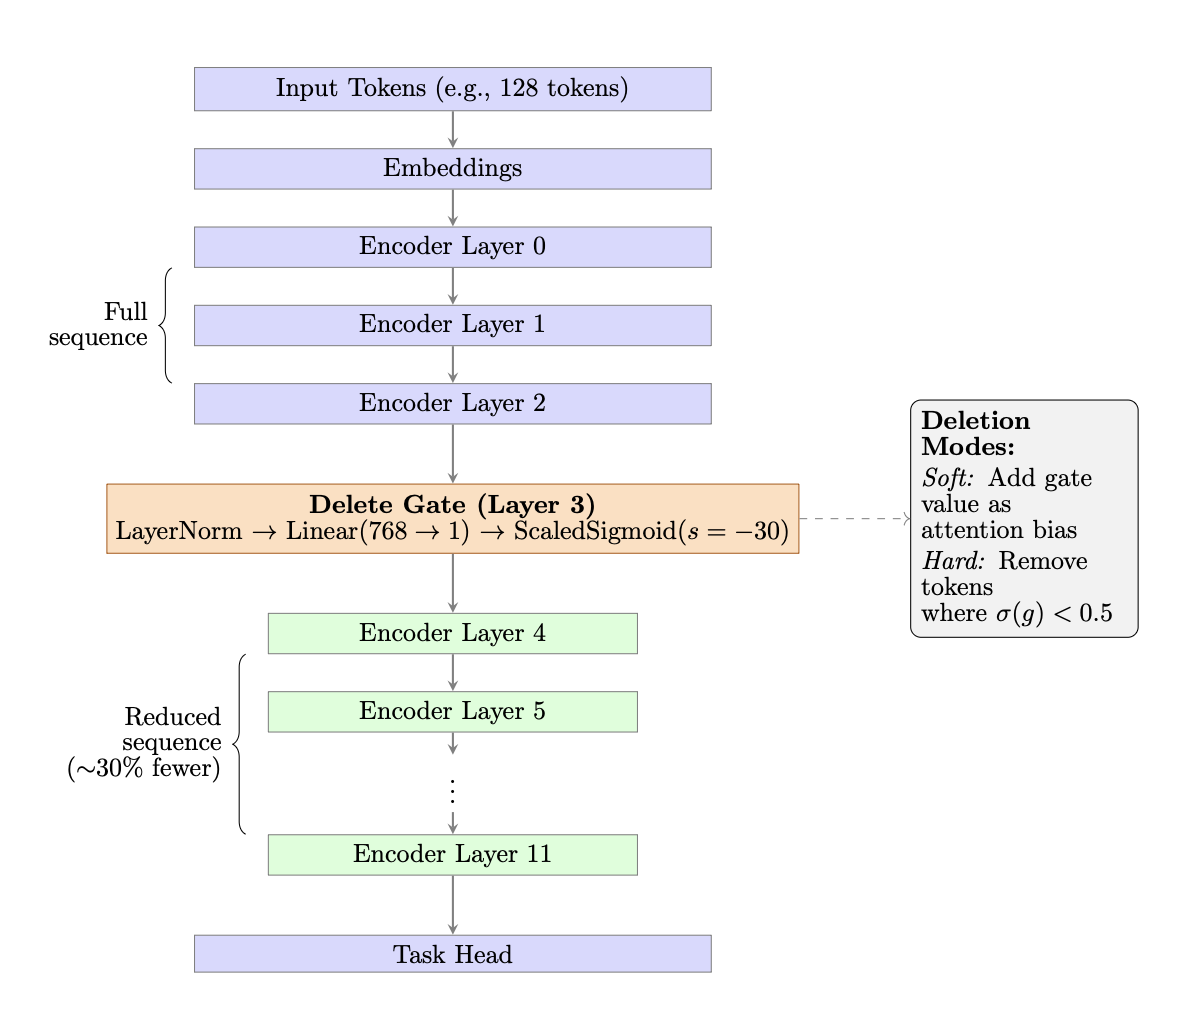
\includegraphics[width=0.55\linewidth]{architecture.png}
  \caption{MrBERT architecture overview. The delete gate at layer 3 
  reduces the sequence length for subsequent layers.}               
  \label{fig:mrbert-arch}                                           
  \end{figure}

\textbf{BERT-base} \citep{devlin2019bert} is a 12-layer encoder with hidden dimension 768, 12 attention heads, 110M parameters, and a 30K WordPiece vocabulary.


\subsection{Pre-deletion blending}
\label{sec:pre-deletion-blending}

For extractive QA, deleted answer tokens produce corrupted representations at the task head. We introduce \textbf{pre-deletion blending}: for each token~$i$, blend weight $w_i = \text{clamp}(-g_i/30,0,1)$, and:
\begin{equation}
    \tilde{\mathbf{h}}_i = (1-w_i)\cdot\mathbf{h}_i^{(L)} + w_i\cdot\mathbf{h}_i^{(\text{gate})}
    \label{eq:blending}
\end{equation}
where $\mathbf{h}_i^{(L)}$ is the layer-11 output and $\mathbf{h}_i^{(\text{gate})}$ is the pre-gate hidden state. For kept tokens ($w_i\approx0$), the representation is unchanged. For deleted tokens ($w_i\approx1$), it falls back to the richer pre-gate representation. This also provides a gradient signal through deleted positions, preventing gate collapse during QA training (Section~\ref{sec:results-tydiqa}).

\subsection{QA span remapping under hard deletion}
\label{sec:span-remapping}

Under hard deletion, the span head operates on a shortened sequence. Predicted start and end indices must be remapped to the original tokenisation for correct evaluation. We maintain a per-example mapping $\texttt{keep\_indices}[b,j]$, recording the original position of the $j$-th kept token in example~$b$, along with $\texttt{kept\_lengths}[b]$. After the span head predicts $(\hat{s},\hat{e})$ in the shortened sequence, we recover original-space positions:
\begin{equation}
    s = \texttt{keep\_indices}[b,\hat{s}], \quad e = \texttt{keep\_indices}[b,\hat{e}]
    \label{eq:span-remap}
\end{equation}
Exact Match is then computed in the original token space. Variable-length sequences within a batch are handled via \texttt{torch.gather} with length masks, producing fixed-shape tensors compatible with standard batched inference.


\subsection{PI controller}
\label{sec:pi-controller}

A PI controller dynamically adjusts the deletion loss coefficient $\alpha$ to track target deletion rate $\delta$:
\begin{align}
    e_t &= \delta - r_t, \quad
    p_t = \gamma p_{t-1} + (1-\gamma)k_p e_t, \quad
    i_t = i_{t-1} + k_i e_t, \quad
    \alpha_t = \max(0, p_t+i_t)
\end{align}
Total loss: $\mathcal{L} = \mathcal{L}_{\text{task}} + \alpha_t\cdot\mathcal{L}_{\text{deletion}}$, where $\mathcal{L}_{\text{deletion}} = \text{mean}(g_i)$ over non-padding tokens. Parameters: $k_p=0.01$, $k_i=10^{-5}$, $\gamma=0.9$.


\subsection{Key differences from MrT5}

Key adaptations from MrT5: (1) the gate fires \emph{after} the full encoder layer (attn + FFN), giving it richer contextual representations; (2) we add pre-deletion blending, which is critical for QA; (3) we use WordPiece tokenisation (30K vocab) rather than byte-level. Full comparison in Table~\ref{tab:diff-mrt5} (Appendix).


% ══════════════════════════════════════════════════════════
\section{Experiments}
\label{sec:experiments}

\subsection{Data}

We evaluate on six datasets: SNLI \citep{bowman2015snli}, SQuAD v1.1 \citep{rajpurkar2016squad}, SST-2 \citep{socher2013sst} and MRPC \citep{dolan2005mrpc} from the GLUE benchmark \citep{wang2019glue}, IMDB \citep{maas2011imdb}, and TyDi~QA \citep{clark2020tydiqa}. Table~\ref{tab:datasets} summarises tasks and splits.

\begin{table}[t]
\centering\small
\begin{tabular}{@{}llrrrl@{}}
\toprule
\textbf{Dataset} & \textbf{Task} & \textbf{Train} & \textbf{Dev} & \textbf{Test} & \textbf{Labels} \\
\midrule
SNLI       & 3-class NLI          & 550K  & 10K  & 9.8K & entail./neutral/contra. \\
SQuAD v1.1 & Extractive QA        & 87K   & 10K  & ---  & span start/end \\
SST-2      & Sentiment            & 67K   & 872  & ---  & positive/negative \\
MRPC       & Paraphrase           & 3.7K  & 408  & 1.7K & equiv./not equiv. \\
IMDB       & Sentiment            & 25K   & 2.5K & 25K  & positive/negative \\
TyDi QA   & Multilingual QA      & 204K  & 9K   & ---  & span (9 languages) \\
\bottomrule
\end{tabular}
\caption{Datasets and task descriptions.}
\label{tab:datasets}
\end{table}

SNLI uses \texttt{max\_seq\_length}=128, SQuAD/TyDi~QA use 384 with stride~128, IMDB uses 512. All datasets are stored as pre-tokenised NDJSON files.


\subsection{Models and baselines}

For each task we train: \textbf{Baseline} (vanilla BERT), \textbf{MrBERT-0\%} (gate active, $\delta=0$; sanity check), \textbf{MrBERT-30\%} (main result), \textbf{MrBERT-50\%/70\%} (SNLI tradeoff curve), \textbf{Random-30\%} (uninformed deletion ablation), \textbf{No-PI-30\%} (fixed $\alpha$ ablation), and \textbf{gate layer ablations} (layers 1, 3, 6, 9 on SNLI).


\subsection{Experimental details}

All models are implemented with HuggingFace Transformers \citep{wolf2020transformers} and Datasets \citep{lhoest2021datasets}, fine-tuned from \texttt{bert-base-uncased} using AdamW, lr=$2\times10^{-5}$, weight decay=0.01, 3 epochs (5 for MRPC). Gate lr=$10^{-4}$. Batch size 32 (classification) / 16 (QA). Regulariser delay: 1,000 steps (100 steps for TyDi~QA). Hard deletion at inference; soft during training. Training on NVIDIA A100 via Modal. Mixed precision (fp16). Seed 42.


\subsection{Results}

\subsubsection{SNLI (natural language inference)}
\label{sec:results-snli}

Table~\ref{tab:snli-results} presents the full SNLI ablation. MrBERT-0\% exactly matches the baseline (90.50\% vs 90.48\%), confirming no architectural overhead. At 30\% deletion, accuracy drops only \textbf{0.27pp} with \textbf{1.89$\times$} speedup (0.763 vs.\ 1.440~ms/sample). Speedup saturates at $\sim$2.05$\times$ beyond 50\% deletion, bounded by fixed pre-gate computation. The accuracy--deletion tradeoff is remarkably linear ($\approx$0.5pp per 10pp deletion).

The random gate achieves only 87.26\% despite nominally targeting 30\% deletion --- it actually deletes 49.6\% because it wastes budget on already-padded positions, producing a much longer average post-deletion sequence (64.2 vs 18.7 tokens). This \textbf{2.95pp gap} between learned and random deletion confirms the gate is learning non-trivial token importance. The random gate also achieves only 1.24$\times$ speedup, highlighting that efficiency gains come from \emph{targeted} deletion of low-content positions, not merely reducing token count.

The No-PI ablation is dramatic: without the controller, the gate runs away to \textbf{89.0\% actual deletion} (target: 30\%), reducing the average sequence to 3.0 tokens and dropping accuracy to 86.47\% --- 3.74pp below the PI-controlled MrBERT-30\% (4.01pp below the BERT baseline).

\begin{table}[t]
\centering
\begin{tabular}{@{}lccccc@{}}
\toprule
\textbf{Model} & \textbf{Accuracy} & \textbf{$\Delta$ (pp)} & \textbf{Del Rate} & \textbf{Avg Seq Len} & \textbf{ms/sample} \\
\midrule
BERT baseline             & 90.48\% & ---     & 0\%     & 27.5  & 1.440 \\
MrBERT 0\% (sanity)      & 90.50\% & $+$0.02 & 0\%     & 27.2  & 0.878$^\dagger$ \\
MrBERT 30\%               & 90.21\% & $-$0.27 & 30.8\%  & 18.7  & 0.763 \\
MrBERT 30\% (hard-train)  & 90.26\% & $-$0.22 & 31.1\%  & 18.9  & 0.757 \\
MrBERT 50\%               & 89.52\% & $-$0.96 & 52.6\%  & 12.9  & 0.701 \\
MrBERT 70\%               & 88.25\% & $-$2.23 & 72.4\%  & 7.5   & 0.705 \\
Random gate 30\%          & 87.26\% & $-$3.22 & 49.6\%  & 64.2* & 1.157 \\
No-PI 30\%                & 86.47\% & $-$4.01 & 89.0\%  & 3.0   & --- \\
\midrule
\multicolumn{6}{@{}l}{\textit{Gate layer ablation (all at 30\% target)}} \\
Layer 1                   & 90.42\% & $-$0.06 & 31.0\%  & 18.9  & 0.568 \\
Layer 3 (default)         & 90.21\% & $-$0.27 & 30.8\%  & 18.7  & 0.761 \\
Layer 6                   & 90.36\% & $-$0.12 & 33.9\%  & 18.1  & 1.039 \\
Layer 9                   & 90.22\% & $-$0.26 & 46.3\%  & 14.6  & 1.324 \\
\bottomrule
\end{tabular}
\caption{SNLI test results. All inputs are padded to 128 tokens. $\Delta$ is relative to the BERT baseline. Runtime measured on NVIDIA A100 with hard deletion. Layer~3 provides the best accuracy--efficiency balance. The No-PI run collapses to 89\% deletion (target: 30\%). *Random gate does not always delete padding, so its Avg Seq Len includes surviving pad tokens (unlike learned-gate rows, which always hard-delete padding). $^\dagger$MrBERT-0\% is faster than BERT despite 0\% non-padding deletion because hard deletion still removes all padding tokens, so post-gate layers process only $\sim$27 tokens instead of 128.}
\label{tab:snli-results}
\end{table}

\begin{figure}[t]
\centering
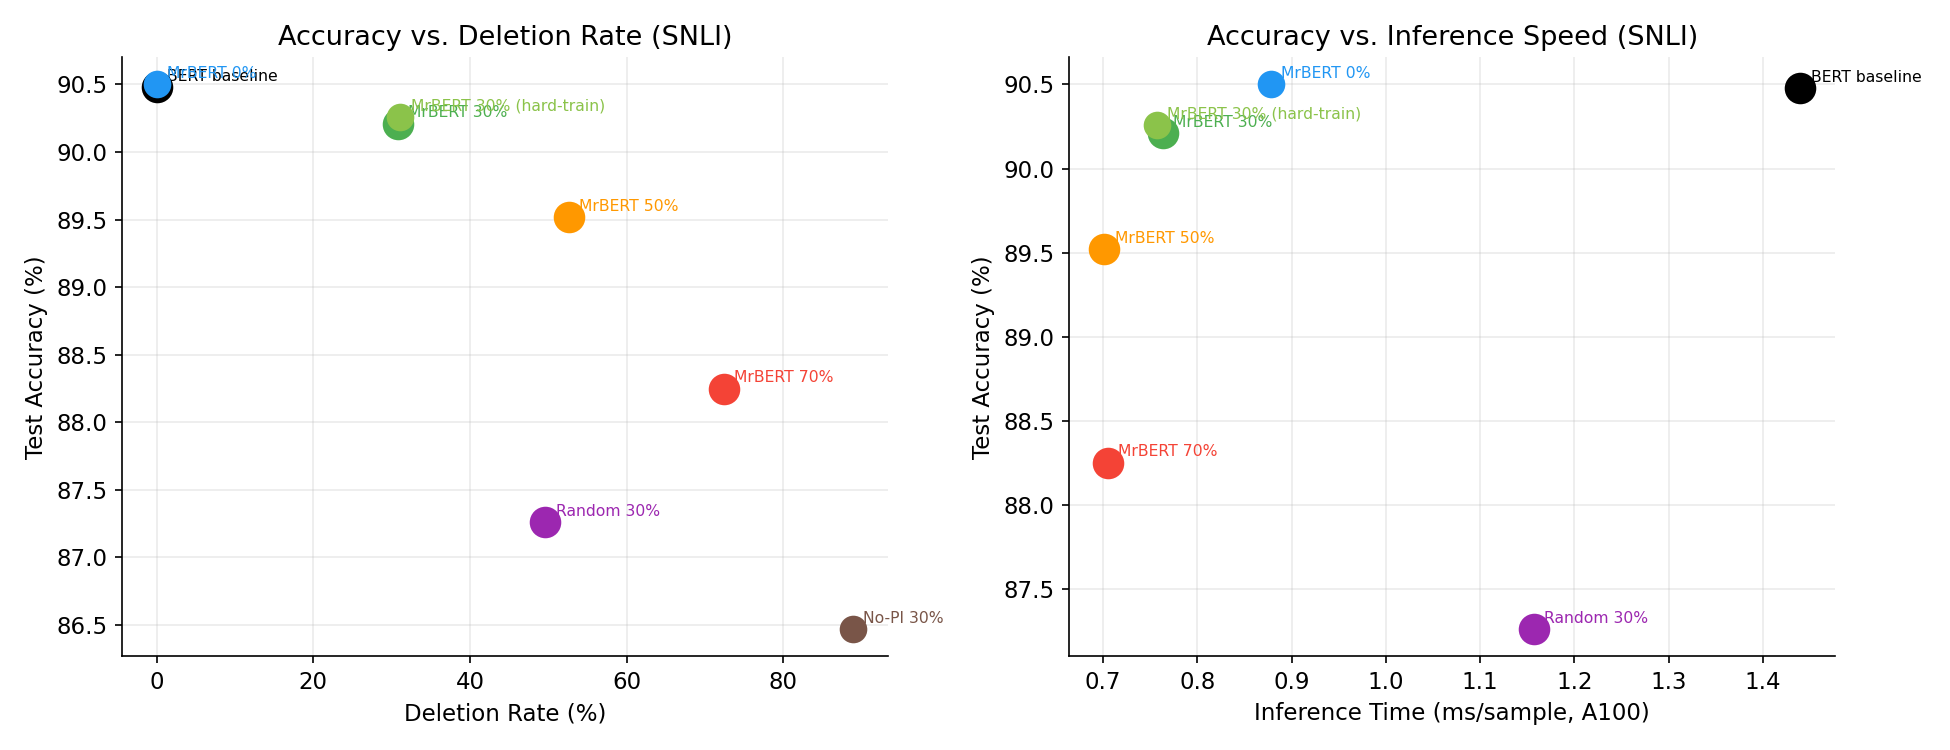
\includegraphics[width=0.55\linewidth]{snli_efficiency_frontier.png}
\caption{SNLI accuracy--efficiency tradeoff. The learned gate consistently dominates the random baseline. Speedup saturates beyond 50\% deletion due to fixed pre-gate computation (layers 0--2 plus the gate). Training curves are in Appendix~\ref{app:training}.}
\label{fig:snli-frontier}
\end{figure}


\begin{figure}[t]
\centering
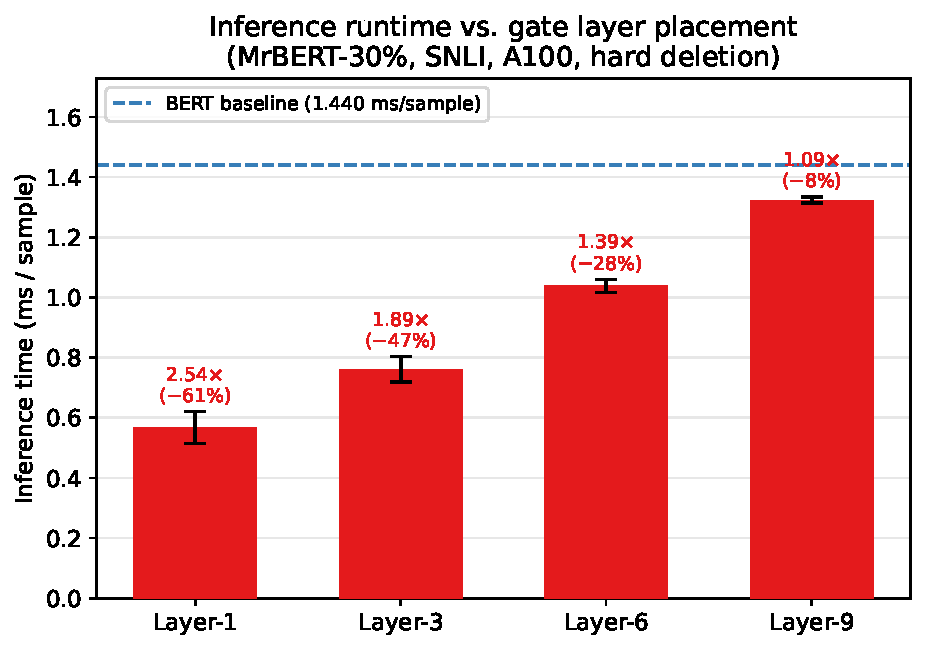
\includegraphics[width=0.55\linewidth]{snli_runtime_vs_deletion_gate_layer.pdf}
\caption{Inference runtime vs.\ gate layer placement (A100, hard deletion). Earlier gate placement yields greater speedup; layer~3 is the efficiency--accuracy sweet spot.}
\label{fig:runtime-gate-layer}
\end{figure}


\subsubsection{SST-2, MRPC, and IMDB}
\label{sec:results-classification}

Table~\ref{tab:classification-results} shows results on three additional tasks. SST-2 and IMDB are highly robust ($-$0.62pp and $-$0.94pp respectively) --- sentiment depends on few keywords, so most tokens are dispensable. IMDB overshoots the 30\% target (actual 43.7\%) because long sequences have noisier per-batch deletion ratios and the PI controller adapts too slowly. MRPC shows a larger $-$15.00pp drop, likely due to its small training set (3.7K examples) making the joint task + deletion objective difficult to optimise. These results reveal a task-sensitivity spectrum: the gate acts as a dynamic regulariser that helps when redundancy is high but harms when critical information is distributed across many positions.

\begin{table}[t]
\centering
\begin{tabular}{@{}lcccccc@{}}
\toprule
\textbf{Dataset} & \textbf{Baseline} & \textbf{MrBERT-30\%} & \textbf{$\Delta$ (pp)} & \textbf{Del Rate} & \textbf{Avg Seq Len} & \textbf{Seq Red.} \\
\midrule
SST-2 & 97.29\% & 96.67\% & $-$0.62 & 47.4\%  & 6.96  & 94.6\%* \\
MRPC  & 83.71\% & 68.71\% & $-$15.00 & 5.7\%   & 50.0  & 60.9\%* \\
IMDB  & 93.97\% & 93.03\% & $-$0.94 & 43.7\%  & 150.8 & 70.6\% \\
\bottomrule
\end{tabular}
\caption{Classification results on SST-2, MRPC, and IMDB. $\Delta$ is relative to the BERT baseline; Del Rate is the fraction of non-padding tokens deleted; Seq Red.\ is the reduction in average sequence length relative to the padded maximum ($1 - \text{Avg Seq Len}/\text{max\_seq\_length}$). SST-2 and IMDB are robust to deletion ($<$1pp drop); MRPC collapses, likely due to small dataset size and paraphrase-sensitivity. *Seq Red.\ includes padding removal (free at inference for all MrBERT variants); for SST-2 and MRPC, padding dominates the reduction --- Del Rate better reflects the gate's learned contribution.}
\label{tab:classification-results}
\end{table}

\subsubsection{SQuAD (extractive QA)}
\label{sec:results-squad}

The SQuAD baseline achieves strong performance (loss 1.076 on the eval set). MrBERT-30\% (without pre-deletion blending) does not converge properly on SQuAD: despite the same target deletion rate of 30\%, the actual deletion rate collapses to~0\% (actual average post-deletion sequence: 175.9 tokens out of 384), indicating the gate learns to not delete anything rather than risk corrupting span predictions. This is analogous to gate collapse observed in TyDi~QA without blending (Section~\ref{sec:results-tydiqa}).


\subsubsection{TyDi QA (multilingual extractive QA)}
\label{sec:results-tydiqa}

Table~\ref{tab:tydiqa-results} (Appendix~\ref{app:tydiqa-results}) shows the progression of our approach. Without pre-deletion blending, the gate collapses to \textbf{60.7\% deletion} at layer~3 (target: 30\%), and span~EM falls to 0.15 (63\% relative drop vs baseline). Pre-deletion blending at layer~3 stabilises deletion at $\sim$0\% (the gate learns to avoid deletion entirely, preserving span integrity), which still improves span~EM to 0.39.

Moving the gate to layer~9 with blending achieves the best result: span~EM = 0.39, start accuracy = 0.53, and end accuracy = 0.49 --- nearly matching BERT baseline (0.40 / 0.53 / 0.50). The actual deletion rate ($\sim$24.7\% non-padding tokens deleted) is close to the 30\% target. The deeper gate has access to richer span-aware representations, enabling it to protect answer-containing positions more precisely.

\begin{figure}[t]
\centering
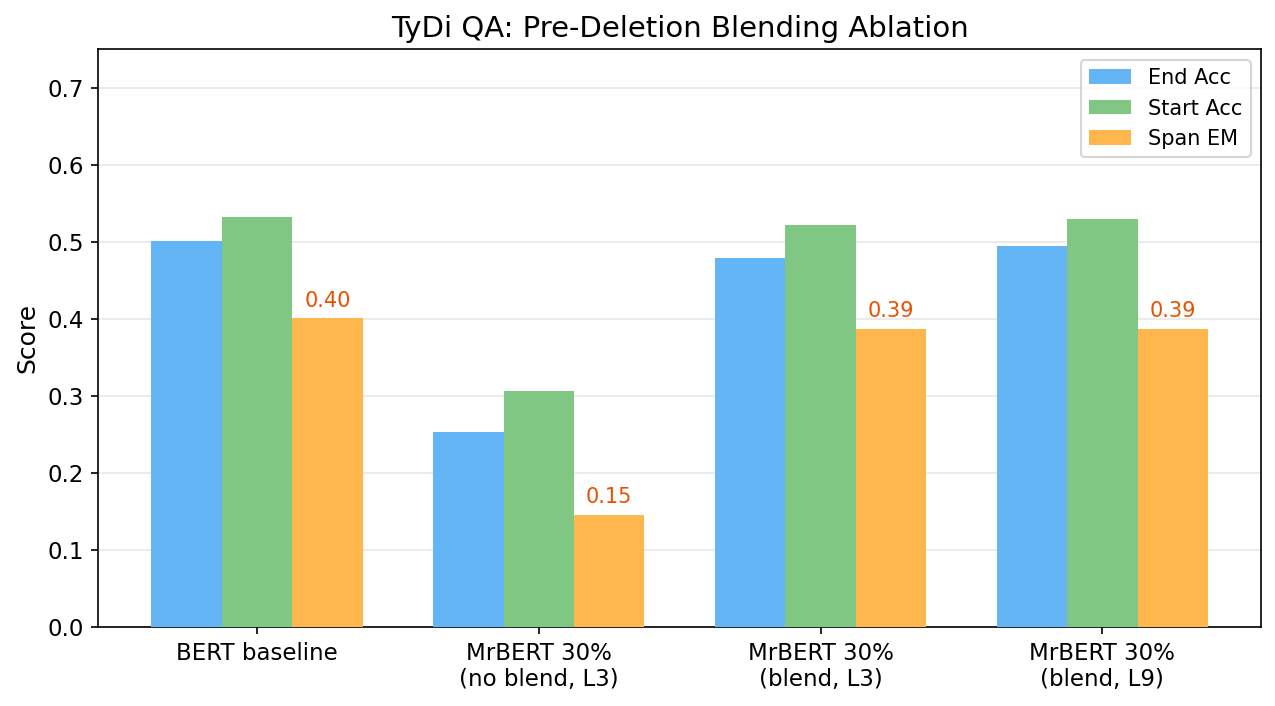
\includegraphics[width=0.55\linewidth]{tydiqa_blending_ablation.png}
\caption{TyDi~QA pre-deletion blending ablation. End accuracy, start accuracy, and span EM for each configuration. Layer~9 with blending nearly closes the gap to BERT baseline.}
\label{fig:tydiqa-ablation}
\end{figure}



% ══════════════════════════════════════════════════════════
\section{Analysis}
\label{sec:analysis}

\subsection{Accuracy--efficiency tradeoff}

The accuracy--efficiency tradeoff on SNLI is remarkably favourable for MrBERT: each 10pp of deletion costs $\approx$0.5pp accuracy. Theoretically, with gate at layer~3 (3 pre-gate layers, 9 post-gate layers) and $k=0.70$ keep ratio:
\begin{equation}
    \text{MACs}_{\text{rel}} = \frac{3 + 9k^2}{12} = \frac{3 + 9\times0.49}{12} \approx 0.62
\end{equation}
yielding 38\% theoretical compute savings. The measured \textbf{47\% runtime reduction} exceeds this because hard deletion also saves memory bandwidth and eliminates FFN computation for deleted positions.

The random gate falls well below the learned frontier (87.26\% at 49.6\% actual deletion vs 90.21\% at 30.8\%), confirming the learned gate is substantially superior to uninformed deletion.


\subsection{PI controller necessity}
\label{sec:pi-necessity}

Without the PI controller, a fixed $\alpha=0.01$ allows the gate to overshoot: actual deletion reaches 89.0\% (target: 30\%), reducing average sequence length to 3.0 tokens and dropping accuracy to 86.47\% --- 3.74pp below PI-controlled MrBERT-30\%. The PI controller prevents this by reducing $\alpha$ when deletion overshoots and increasing it when undershooting, achieving stable convergence within the first epoch (see Appendix~\ref{app:training} for dynamics).


\subsection{Soft--hard deletion gap}

The soft--hard gap is only \textbf{0.05pp} for soft-only training, and \textbf{0.01pp} for hard-train (trained with \texttt{hard\_delete\_train\_prob}=0.5). This validates the core design: soft deletion during training is sufficient for hard-deletion robustness at inference (see Appendix~\ref{app:training} for training curves).




\subsection{Token deletion patterns}
\label{sec:deletion-patterns}

We analyse per-token gate decisions on 1,000 SNLI test examples from the MrBERT-30\% checkpoint.
Overall accuracy on this sample: 89.80\% (898/1000).
Per-class: contradiction 94.83\% (312/329), entailment 90.41\% (311/344), neutral 84.10\% (275/327).

\begin{figure}[t]
\centering
\begin{minipage}[b]{0.49\textwidth}\centering
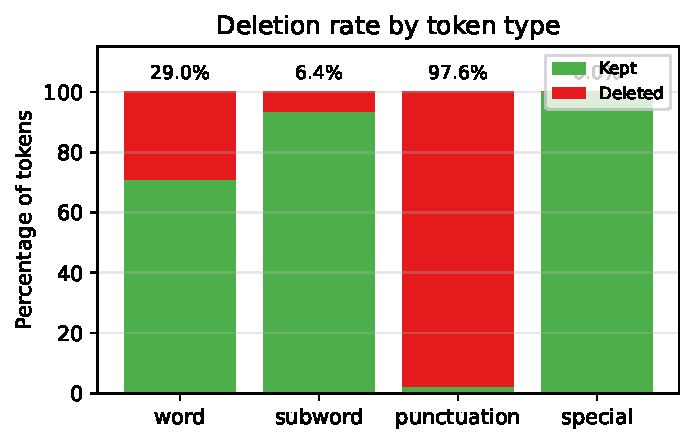
\includegraphics[width=\linewidth]{mrbert-snli-30pct_test_by_type.pdf}
\end{minipage}\hfill
\begin{minipage}[b]{0.49\textwidth}\centering
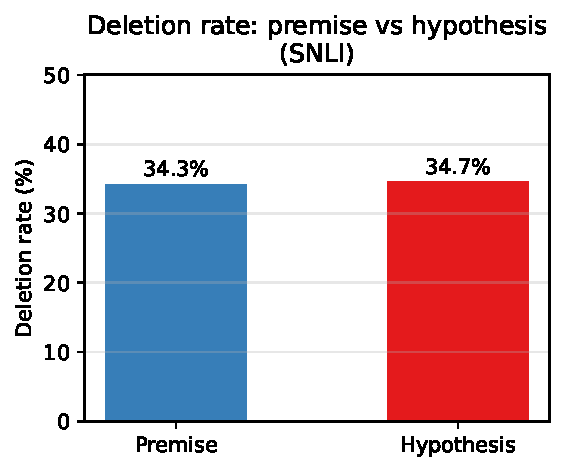
\includegraphics[width=\linewidth]{mrbert-snli-30pct_test_premise_vs_hyp.pdf}
\end{minipage}
\caption{Token deletion pattern analysis on SNLI test set (MrBERT-30\%). Left: Deletion rate by token type. Punctuation is almost universally deleted; subword continuations are preserved. Right: Deletion rate: premise vs.\ hypothesis. Rates are nearly uniform across segments.}
\label{fig:deletion-patterns}
\end{figure}

\textbf{By token type} (Figure~\ref{fig:deletion-patterns}, left). The gate makes sharp type-aware decisions: punctuation is almost universally deleted (97.6\%), whole words are deleted at a moderate rate (29.0\%), subword continuations are rarely deleted (6.4\%, preserving word integrity), and special tokens (\texttt{[CLS]}, \texttt{[SEP]}) are never deleted (0\%). The mean gate value is $-25.58$, with a median of $-30.0$, confirming a strongly bimodal distribution.

\textbf{Premise vs.\ hypothesis} (Figure~\ref{fig:deletion-patterns}, right). Deletion rates are nearly uniform across premise (34.3\%) and hypothesis (34.7\%) segments, indicating the gate does not exhibit segment-level positional bias and instead makes token-level decisions based on content.

\textbf{Deletion by label} (Figure~\ref{fig:deletion-by-label}). Contradiction examples show the highest accuracy (94.8\%) and a bimodal gate distribution; entailment (90.4\%) and neutral (84.1\%) examples show progressively lower accuracy. Deletion rates are nearly uniform across all three labels ($\mu$=29.9--30.8\%), indicating the gate does not preferentially delete based on label difficulty.


\subsection{Per-example degradation analysis}
\label{sec:loss-deletion-correlation}

Does the gate disproportionately harm examples where it deletes more tokens? We compute per-example \emph{delta-loss} (MrBERT loss $-$ BERT baseline loss) on the SNLI validation set (1,000 examples), isolating the causal effect of deletion from inherent example difficulty.

The learned gate shows Pearson $r=-0.018$ ($p=0.58$): deletion rate has \textbf{no relationship} to degradation (Figure~\ref{fig:delta-correlation}). The random deletion baseline is equally flat ($r=-0.009$, $p=0.78$). This contrasts with MrT5, where random byte deletion showed $r=0.295$ --- higher deletion caused proportionally more degradation. The difference suggests subword-level NLI is fundamentally more redundant than byte-level language modelling: even uninformed deletion does not systematically hurt high-deletion examples.

If both show $r\approx0$, what distinguishes the learned gate? The \emph{aggregate} accuracy gap: 62.8\% of examples are worse under the learned gate vs.\ 74.5\% under random, and the learned gate's mean $\Delta$-loss is smaller (+0.075 vs.\ +0.057 for random at 51\% deletion). The gate's value is in \emph{which} tokens it selects, not in varying how many it deletes per example.

\begin{figure}[t]
\centering
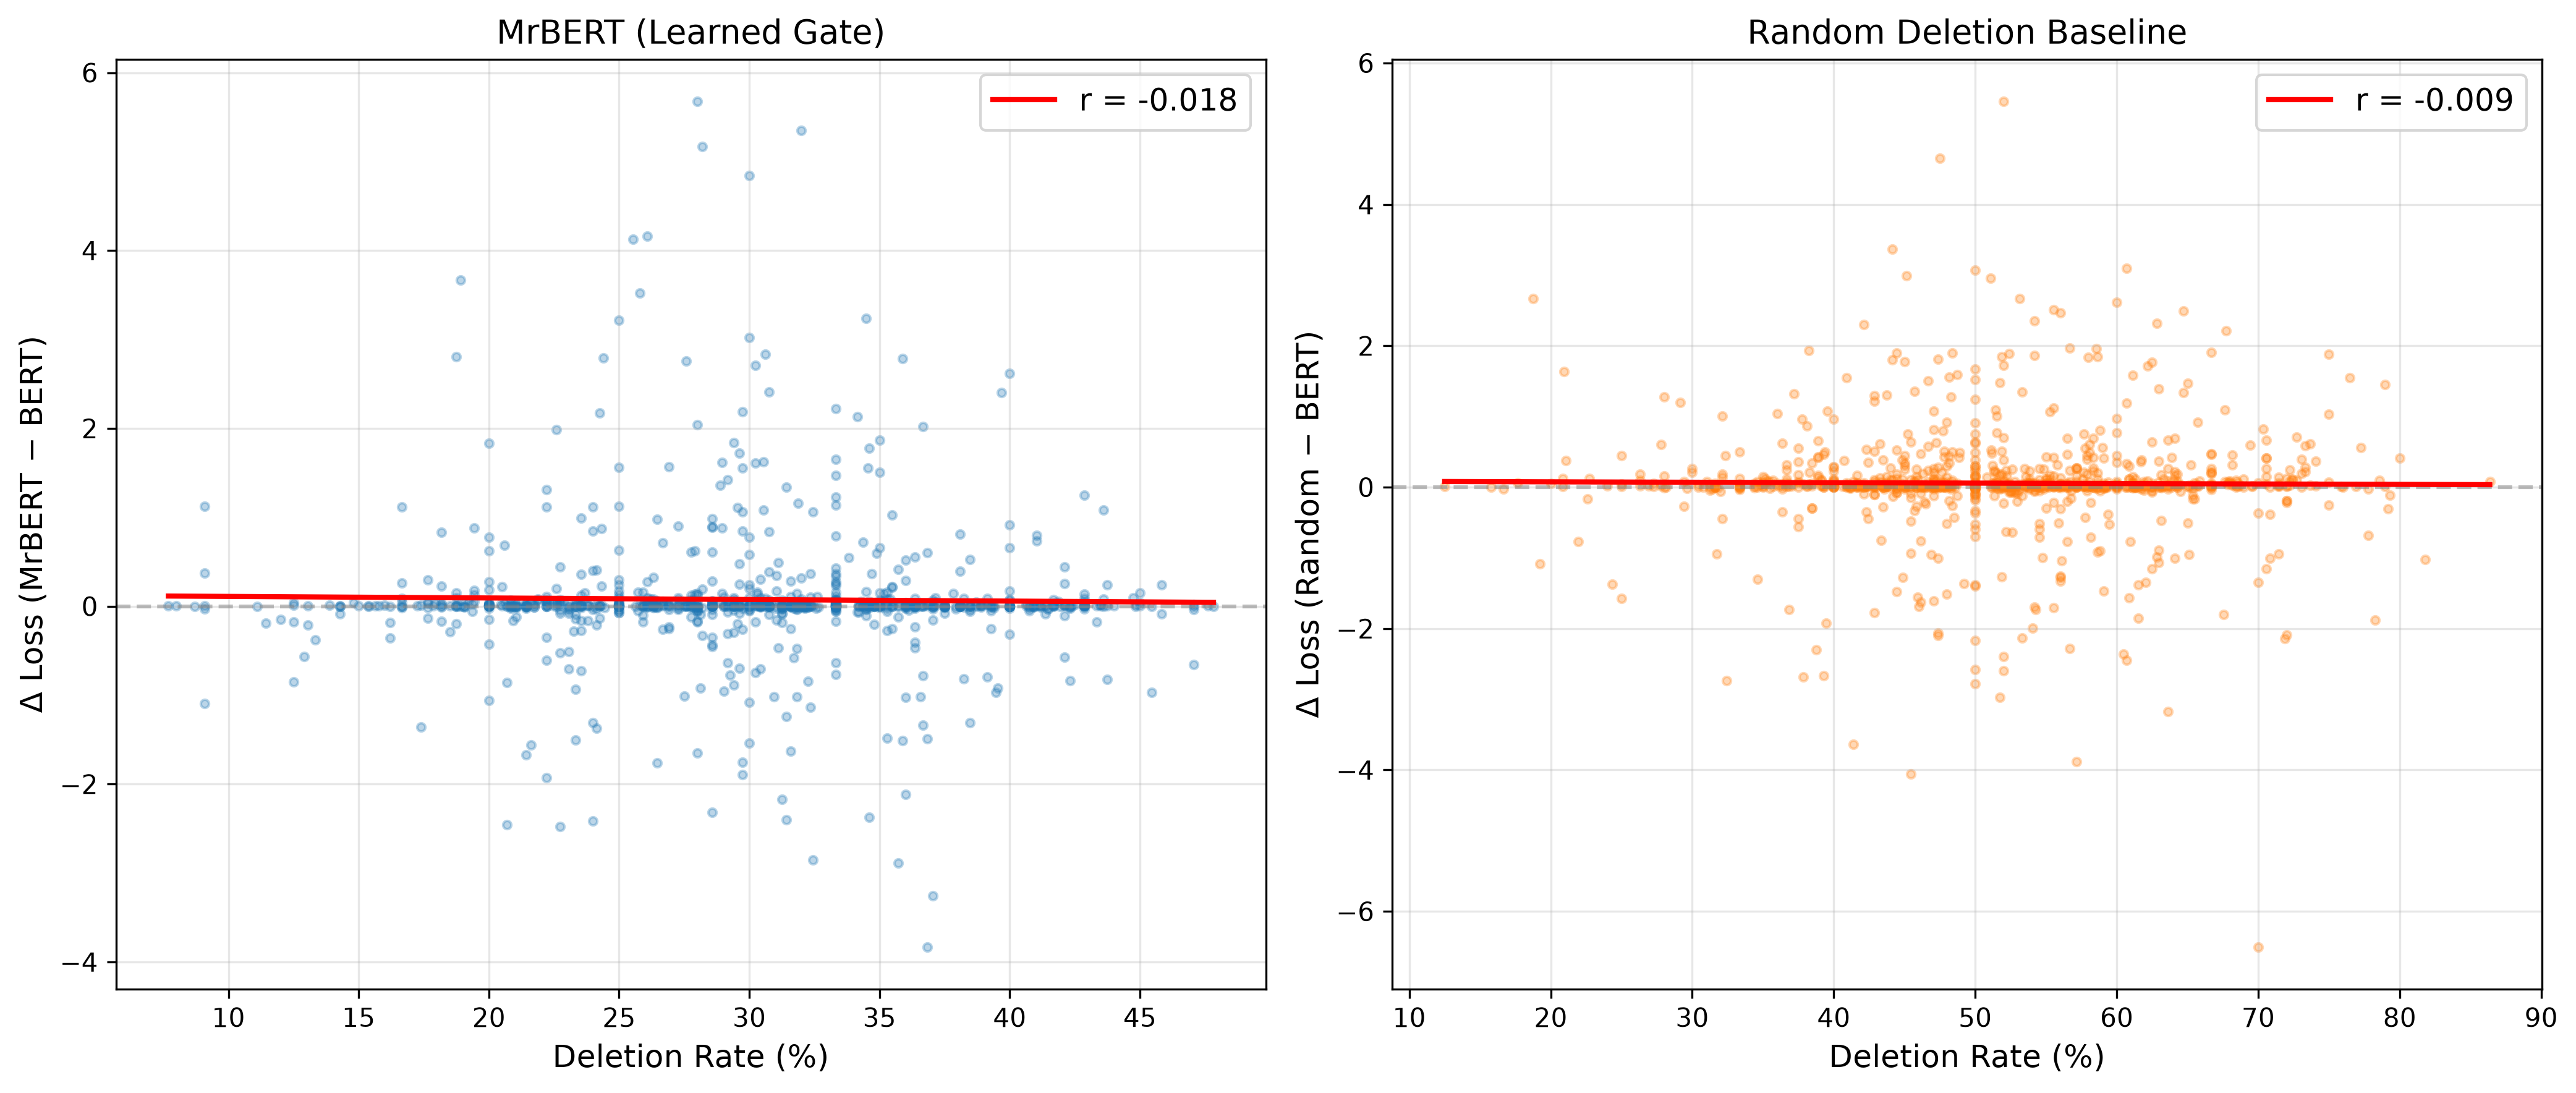
\includegraphics[width=0.95\linewidth]{delta_correlation_scatter.png}
\caption{Per-example $\Delta$-loss (model $-$ BERT baseline) vs.\ deletion rate on SNLI (1,000 validation examples). Left: MrBERT learned gate ($r=-0.018$). Right: Random deletion baseline ($r=-0.009$). Both are flat, but MrT5 found $r=0.295$ for random byte deletion --- subword NLI is more deletion-tolerant than byte-level LM.}
\label{fig:delta-correlation}
\end{figure}


\subsection{Gate layer ablation}

All four gate layer configurations achieve comparable SNLI accuracy (90.21--90.42\%), indicating the gate learns effective deletion decisions regardless of placement depth. However, runtime varies substantially: layer~1 achieves 0.568~ms/sample (2.54$\times$ speedup, 11 of 12 layers run on reduced sequence) while layer~9 achieves 1.324~ms/sample (1.09$\times$ speedup, only 3 layers benefit).

Interestingly, layer~9 achieves a \textbf{higher actual deletion rate} (46.3\%) despite the same 30\% target. Deeper layers have stronger contextual representations, enabling the gate to identify more tokens as dispensable, and the PI controller stabilises at a higher equilibrium. Layer~3 is the sweet spot: strong accuracy, 1.89$\times$ speedup, and 9 downstream layers benefiting from reduced sequence length.


\subsection{Pre-deletion blending: mechanism analysis}

Pre-deletion blending is critical for QA but has no effect on classification (since \texttt{[CLS]} always has $g=0$, the blend weight is 0 for the pooled output).

For TyDi~QA, the mechanism addresses two distinct failure modes:
\begin{enumerate}[nosep]
    \item \textbf{Gate collapse} (without blending): the gradient signal through deleted positions is corrupted; the gate destabilises and overshoots to 60.7\% deletion, deleting many answer tokens.
    \item \textbf{Representation corruption} (with blending but wrong layer): at layer~3 with blending, the gate stabilises at 0\% deletion (it learns to keep everything), recovering span EM to 0.39 but sacrificing efficiency.
\end{enumerate}

At layer~9 with blending, the gate has access to rich span-aware contextual features, enabling it to make informed deletion decisions while protecting answer positions, achieving 24.7\% actual deletion and span EM 0.39. The gate std dev (10.3 at layer~9 vs.\ flat~8 without blend) confirms a healthy bimodal distribution.


\subsection{Comparison to MrT5}

MrBERT tolerates 30\% subword deletion with only 0.27pp accuracy loss and 1.89$\times$ speedup --- exceeding MrT5's $\sim$1.3--1.5$\times$ at equivalent deletion --- despite subword tokens being more informationally dense than bytes. The soft--hard gap is only 0.05pp (vs.\ $<$1pp in MrT5). Full comparison in Table~\ref{tab:comparison-mrt5} (Appendix).

% ══════════════════════════════════════════════════════════
\section{Other Related Work}
\label{sec:related-work}

\textbf{Efficient transformers.} Sparse attention \citep{beltagy2020longformer,zaheer2020bigbird}, low-rank projections \citep{wang2020linformer}, kernel methods \citep{choromanski2021performer}, and early-exit approaches \citep{xin2020deebert,zhou2020pabee} all reduce transformer cost. Token pruning methods \citep{ye2021trbert,wang2021spatten,kim2022ltp} learn to drop tokens but often require reinforcement learning. Our method keeps network depth fixed, reduces tokens in later layers via differentiable soft deletion, and requires no architectural changes beyond the gate.

\textbf{Token importance.} \citet{michel2019heads} and \citet{voita2019heads} showed many BERT attention heads are redundant. \citet{clark2019attention} found attention aligns with syntactic structure, with function words receiving less attention in higher layers --- consistent with our gate's deletion patterns (Section~\ref{sec:deletion-patterns}).

\textbf{Summary of differences.} Our work differs from prior token pruning by: (1)~applying dynamic merging to encoder-only architectures; (2)~using a PI controller to stabilise deletion; (3)~introducing pre-deletion blending for extractive QA; and (4)~providing multi-task analysis to identify where merging helps or hurts.

% ══════════════════════════════════════════════════════════
\section{Conclusion}
\label{sec:conclusion}

We have demonstrated that the Dynamic Token Merging delete gate from MrT5 transfers to encoder-only discriminative NLU models. MrBERT learns to selectively delete tokens at controlled rates while preserving task performance. 

\noindent\textbf{Key findings:}

\begin{enumerate}[nosep]
    \item \textbf{Minimal accuracy cost (SNLI)}: MrBERT-30\% retains 90.21\% accuracy --- only 0.27pp below BERT baseline --- at \textbf{1.89$\times$} A100 speedup.
    \item \textbf{Task-dependent robustness}: SST-2 ($-$0.62pp) and IMDB ($-$0.94pp) are highly robust; MRPC ($-$15.00pp) is sensitive, likely due to small dataset size.
    \item \textbf{Learned importance}: gate outperforms random deletion by 2.95pp on SNLI and preferentially deletes punctuation while preserving subword continuations and special tokens.
    \item \textbf{PI controller is essential}: without it, the gate runs away to 89\% deletion, dropping accuracy 4.01pp below the BERT baseline.
    \item \textbf{Pre-deletion blending enables QA}: span EM $0.15\to0.39$ ($2.6\times$); nearly matches BERT baseline at layer~9.
    \item \textbf{Soft training $\Rightarrow$ hard inference}: soft--hard gap is only 0.05pp, validating the training design.
\end{enumerate}

\noindent \textbf{Limitations and future work.}
Hard deletion breaks batch uniformity, complicating deployment.  MRPC's large drop ($-$15.00pp) warrants investigation into small-dataset sensitivity.  Promising extensions include applying pre-deletion blending to SQuAD, cross-lingual transfer via multilingual encoders, and alignment with human-annotated rationales.

\bibliography{references}
\bibliographystyle{colm2026_conference}

\newpage
\appendix

\section*{Appendix}

\section{LLM usage statement}

In accordance with the COLM 2026 policy on the use of large language models, we disclose that LLM-based tools were used to assist with code implementation and with the writing and formatting of this paper, including grammar, phrasing, and conformance to the COLM template. LLMs were not used to originate the research problem, design the experiments, or generate any data, charts, or figures reported in this paper. All references were verified by the authors against their original sources, and the authors have reviewed all LLM-assisted content and take full responsibility for the contents of this paper.

\section{Architecture and design}
\label{app:params}

\begin{table}[H]
\centering
\begin{tabular}{@{}lr@{}}
\toprule
\textbf{Component} & \textbf{Parameters} \\
\midrule
BERT-base                        & 110M \\
Gate LayerNorm (weight $+$ bias)  & $2 \times 768 = 1{,}536$ \\
Gate Linear (weights $+$ bias)    & $768 + 1 = 769$ \\
\textbf{Total gate}               & \textbf{2,305} \\
Gate as \% of BERT-base          & 0.0021\% \\
\bottomrule
\end{tabular}
\caption{Gate module parameter counts.}
\label{tab:params}
\end{table}

\begin{figure}[H]
  \centering
  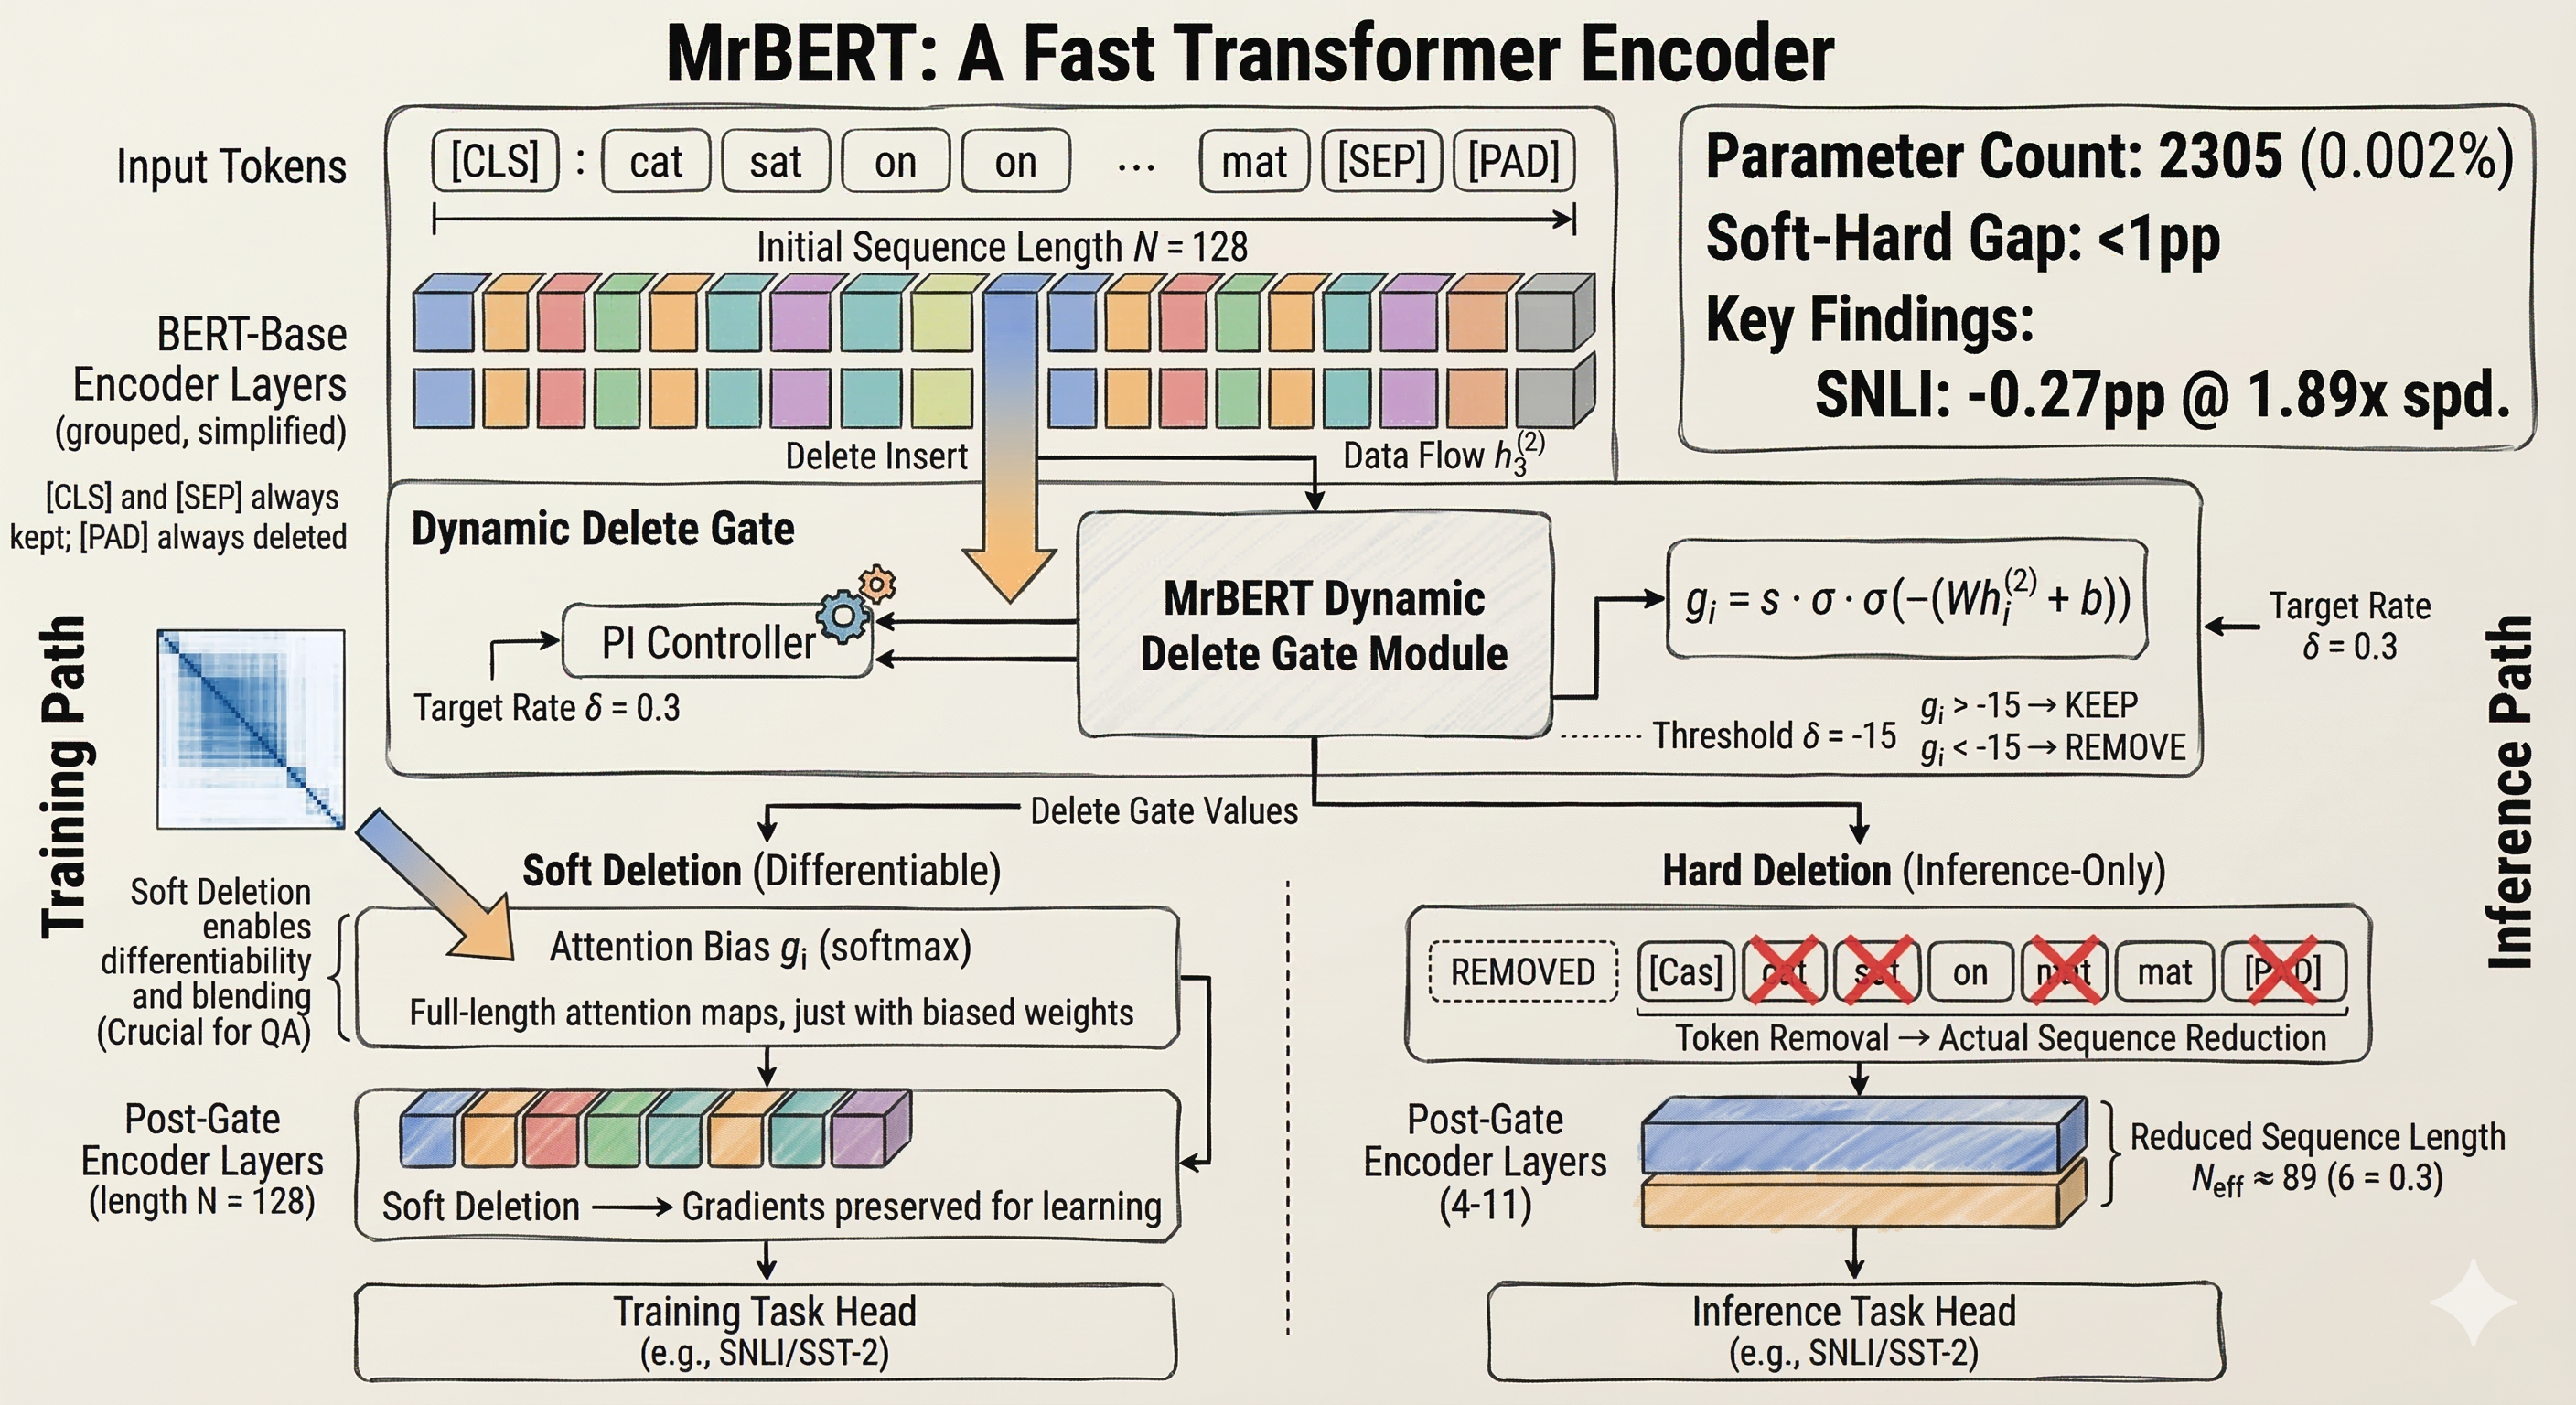
\includegraphics[width=0.55\linewidth]{architecture2.png}
  \caption{Layer-level view of MrBERT. Encoder layers 0--2 (blue) process the full sequence; the delete gate fires at the boundary before layer~3 (orange), and layers 3--11 (green) operate on the reduced sequence ($\sim$30\% fewer tokens at $\delta{=}0.3$). Soft deletion adds gate values as attention biases; hard deletion physically removes tokens where $g < \tau$.}
  \label{fig:mrbert-layers}
\end{figure}

\begin{table}[H]
\centering\small
\begin{tabular}{@{}lll@{}}
\toprule
\textbf{Aspect} & \textbf{MrT5} & \textbf{MrBERT} \\
\midrule
Architecture       & Encoder-decoder (T5)    & Encoder-only \\
Tokenisation       & Byte-level (256 vocab)  & WordPiece 30K \\
Gate fires         & Before self-attention   & After full encoder layer (attn $+$ FFN) \\
Pre-deletion blend & None                    & Yes --- critical for QA \\
Gate init (bias)   & Xavier $+$ $b=1$        & $\mathcal{N}(0,0.02)$ $+$ $b=10.0$ \\
Softmax1           & Off by default          & On by default \\
\bottomrule
\end{tabular}
\caption{Key design differences between MrT5 and our models.}
\label{tab:diff-mrt5}
\end{table}


\section{Training and convergence}
\label{app:training}

\begin{figure}[H]
\centering
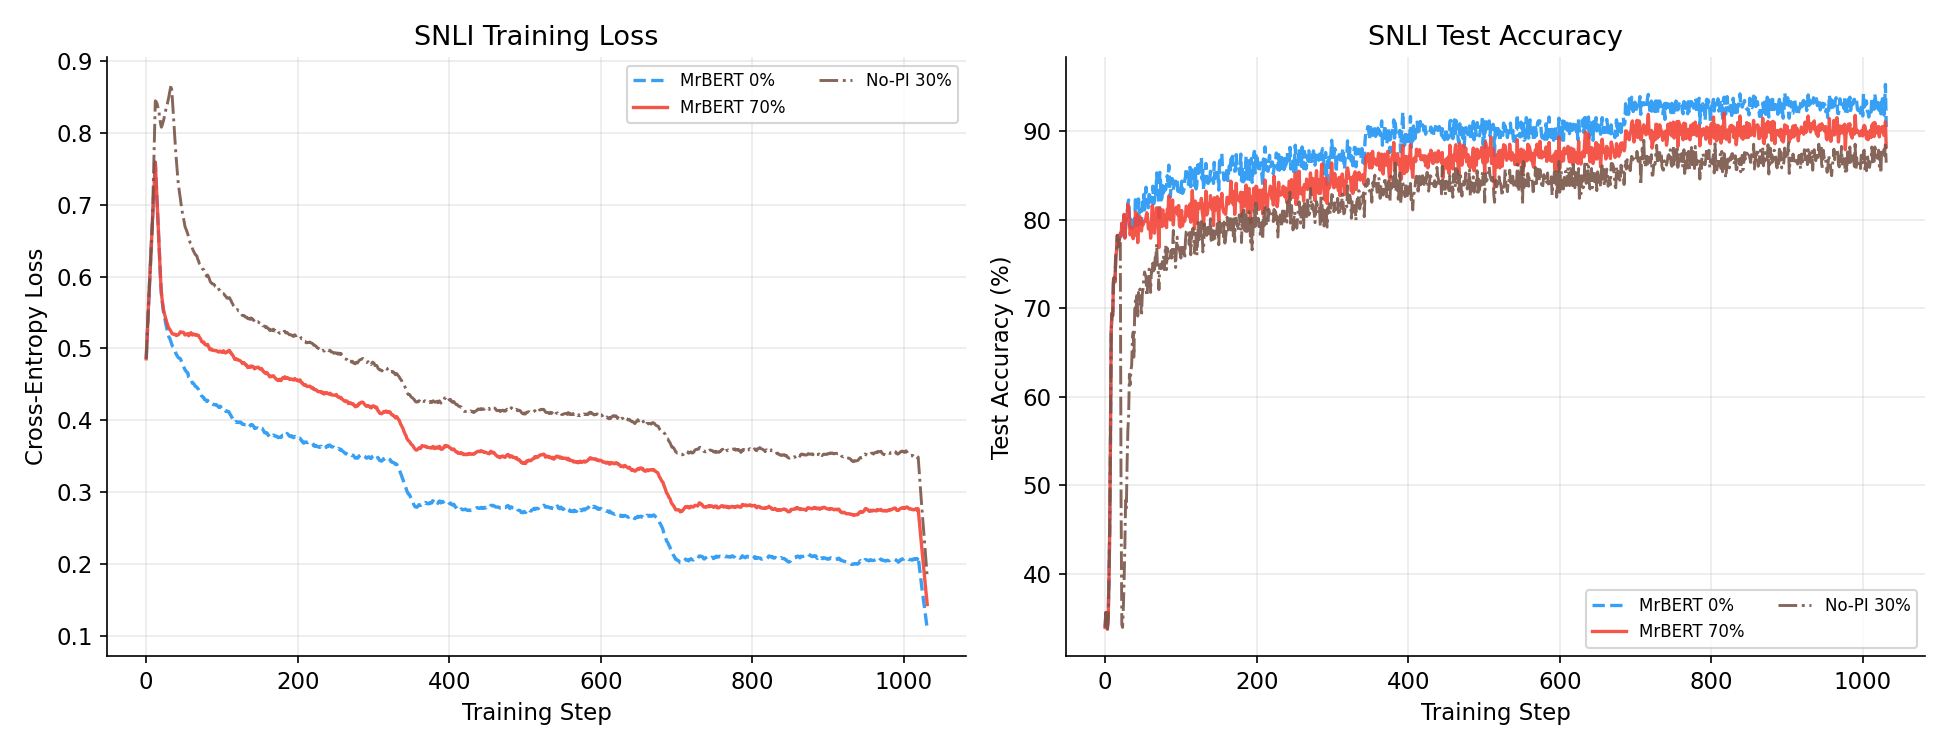
\includegraphics[width=0.55\linewidth]{snli_loss_and_accuracy.png}
\caption{SNLI training loss and test accuracy curves for all model variants.}
\label{fig:snli-training-curves}
\end{figure}

\begin{figure}[H]
\centering
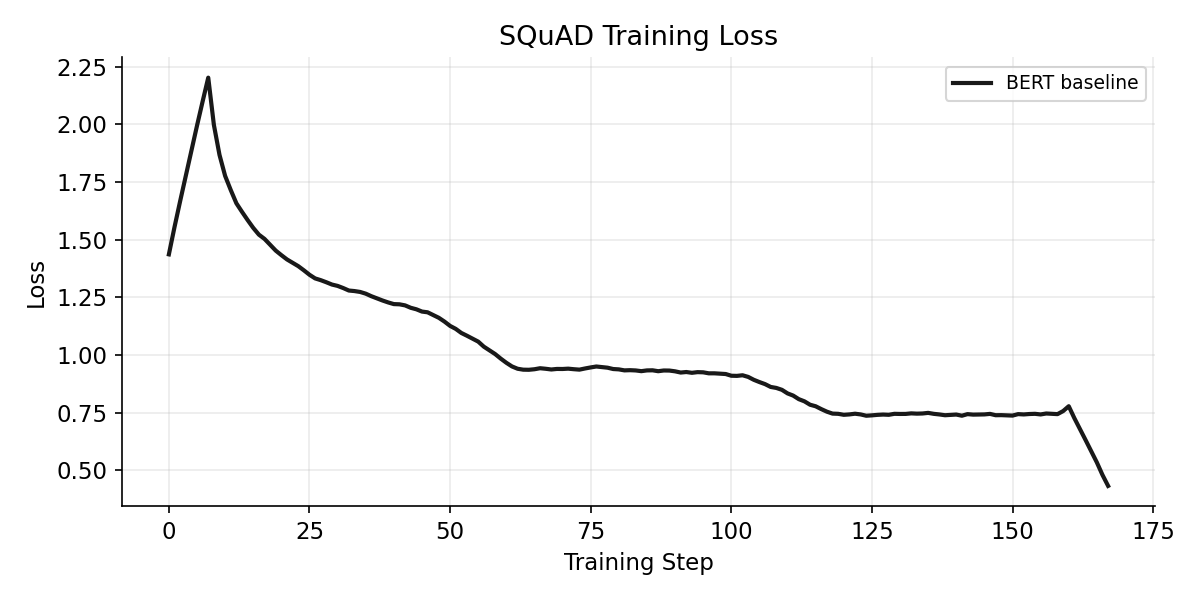
\includegraphics[width=0.55\linewidth]{squad_training_loss.png}
\caption{SQuAD training loss for the BERT baseline. The model converges normally over $\sim$170 steps, reaching a final loss of $\sim$0.75.}
\label{fig:squad-loss}
\end{figure}

\begin{figure}[H]
\centering
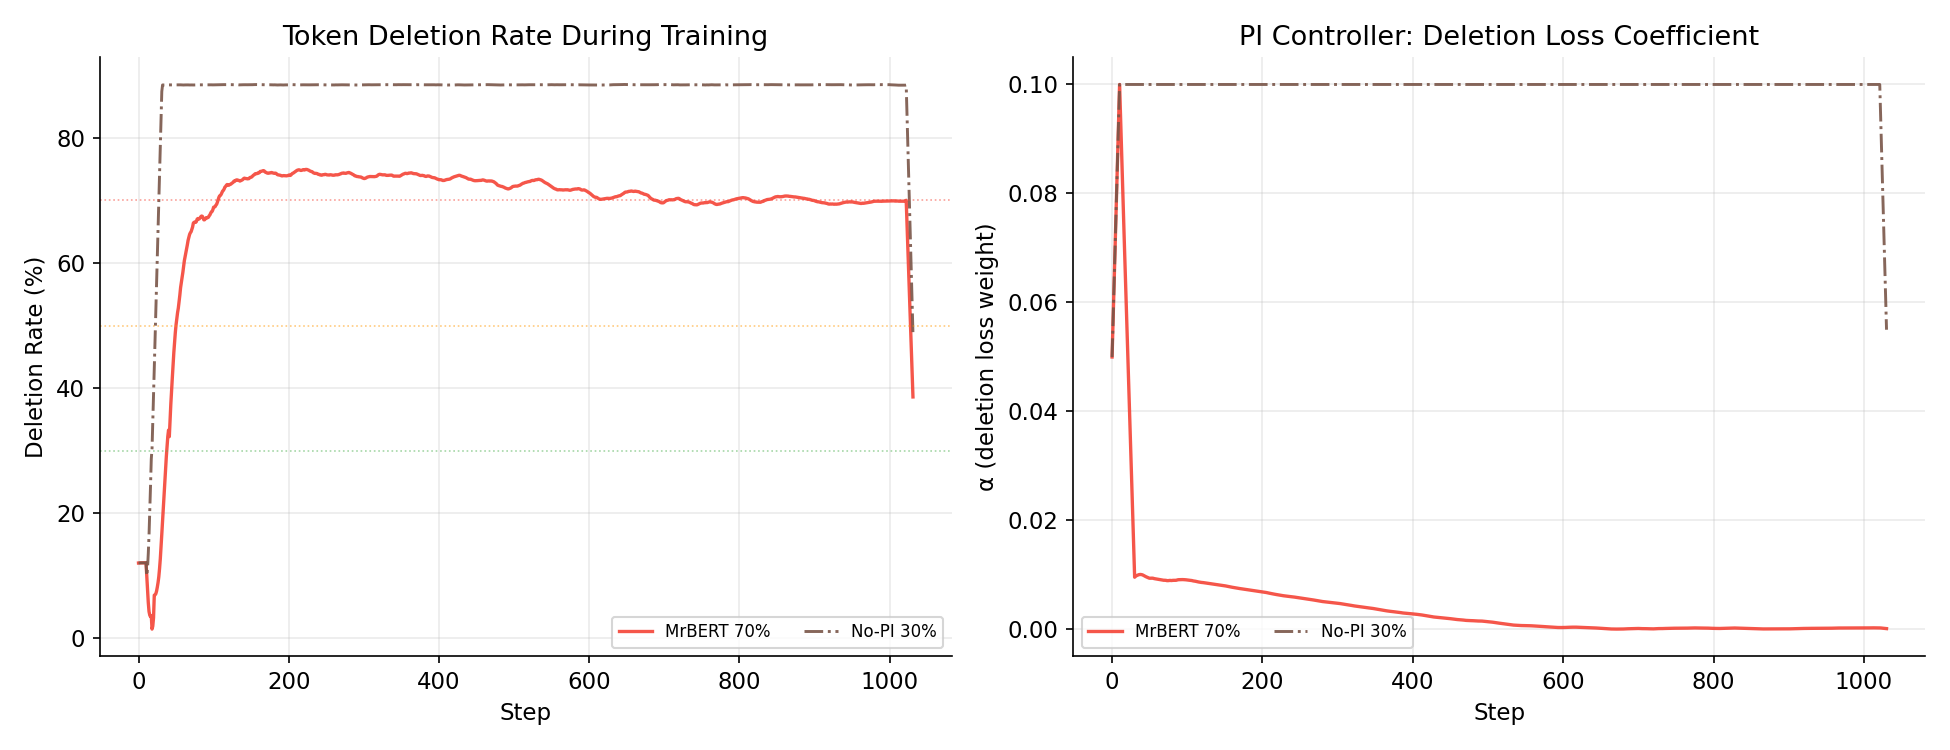
\includegraphics[width=0.55\linewidth]{snli_deletion_and_pi.png}
\caption{Left: deletion rate curves during training. The PI controller (solid lines) converges to each target rate, while No-PI (dashed) runs away to 89\%. Right: the PI controller's $\alpha$ coefficient dynamically adjusts to stabilise deletion.}
\label{fig:pi-controller}
\end{figure}

\begin{figure}[H]
\centering
\begin{minipage}[b]{0.49\textwidth}\centering
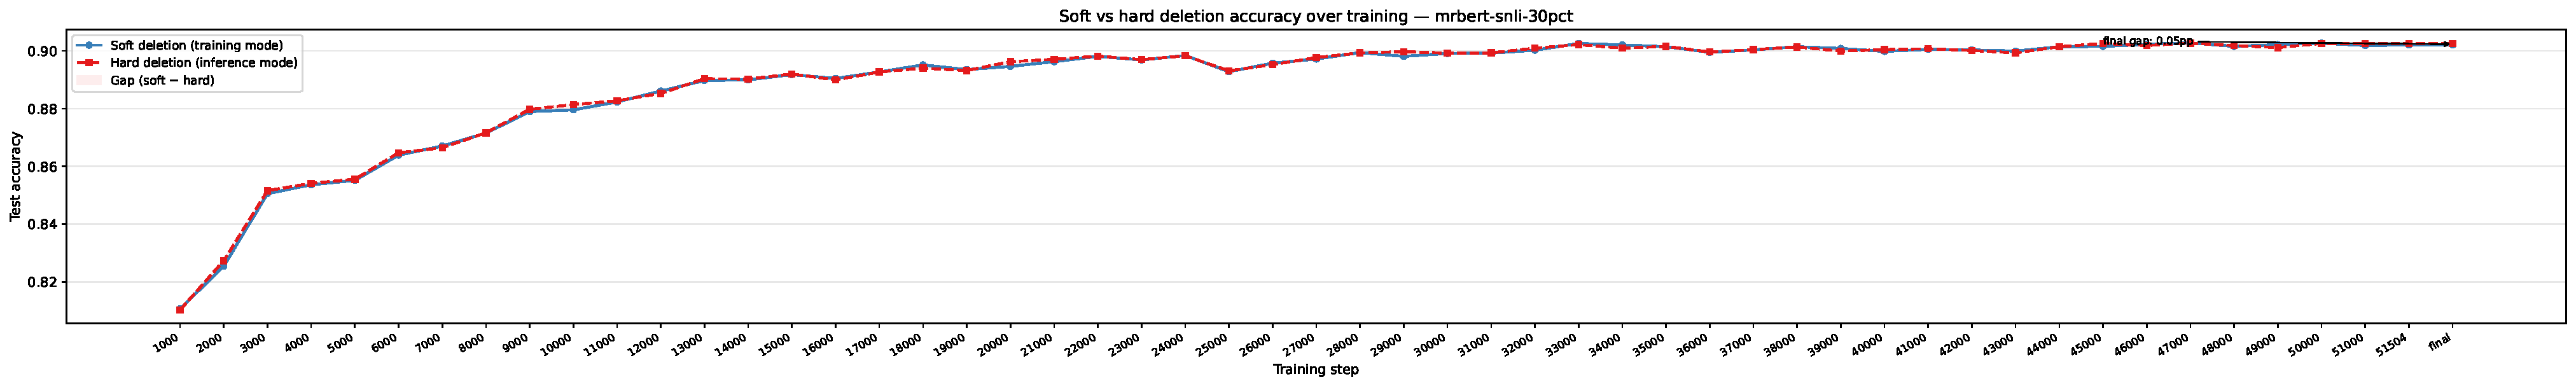
\includegraphics[width=\linewidth]{mrbert-snli-30pct_hard_deletion_curve.pdf}
\end{minipage}\hfill
\begin{minipage}[b]{0.49\textwidth}\centering
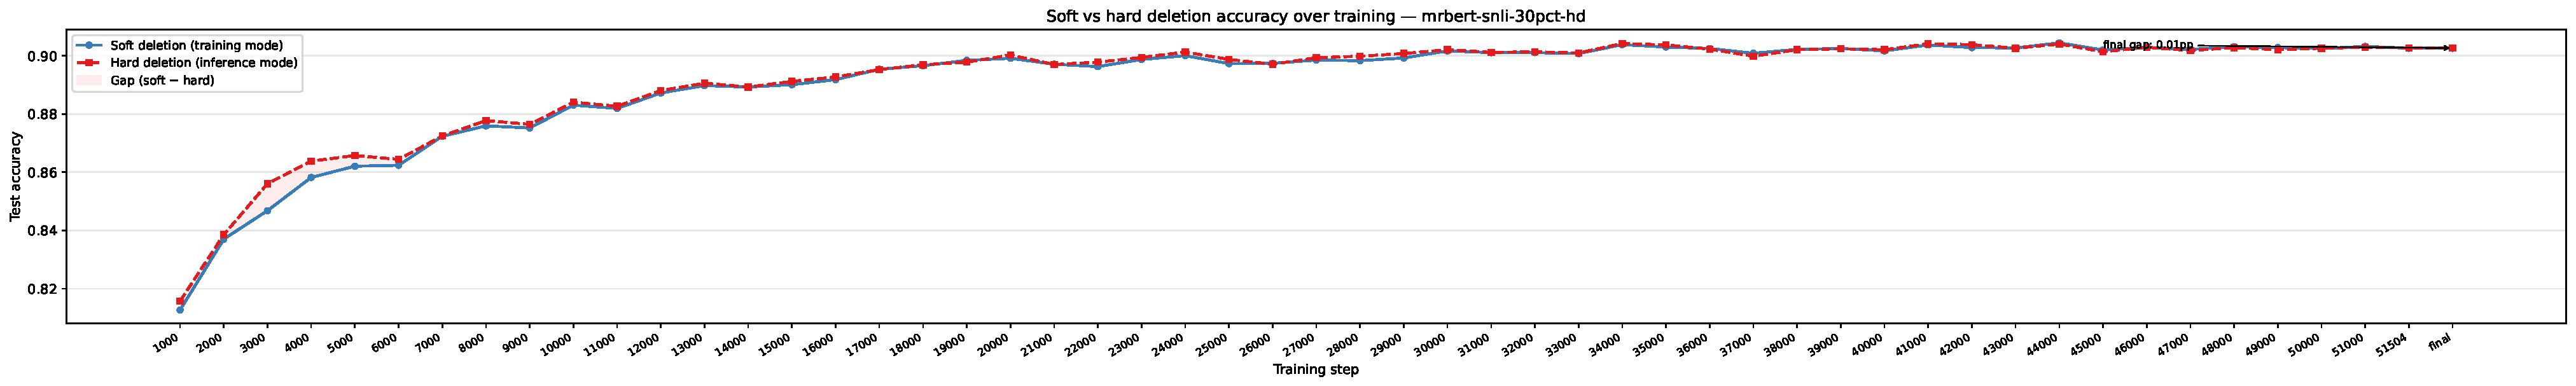
\includegraphics[width=\linewidth]{mrbert-snli-30pct-hd_hard_deletion_curve.pdf}
\end{minipage}
\caption{Soft vs.\ hard deletion accuracy throughout training on SNLI. Both curves track each other tightly. Left: Soft-only training (run~C). Final gap: 0.05pp. Right: Hard-train ($p=0.5$, run~M). Final gap: 0.01pp.}
\label{fig:hard-deletion}
\end{figure}


\section{Extended results}
\label{app:extended-results}

Table~\ref{tab:cross-task-summary} consolidates MrBERT-30\% results across all tasks, providing a single reference point for accuracy, deletion behaviour, and task sensitivity.

\begin{table}[H]
\centering\small
\begin{tabular}{@{}llcccc@{}}
\toprule
\textbf{Task} & \textbf{Metric} & \textbf{Baseline} & \textbf{MrBERT-30\%} & \textbf{$\Delta$} & \textbf{Actual Del.} \\
\midrule
SNLI          & Accuracy  & 90.48\% & 90.21\% & $-$0.27pp  & 30.8\% \\
SST-2         & Accuracy  & 97.29\% & 96.67\% & $-$0.62pp  & 47.4\% \\
IMDB          & Accuracy  & 93.97\% & 93.03\% & $-$0.94pp  & 43.7\% \\
MRPC          & Accuracy  & 83.71\% & 68.71\% & $-$15.00pp & 5.7\%  \\
TyDi QA (L9)  & Span EM   & 0.40    & 0.39    & $-$0.01    & 24.7\% \\
SQuAD$^\dagger$ & ---     & loss 1.08 & gate collapse & ---  & $\sim$0\% \\
\bottomrule
\end{tabular}
\caption{Consolidated MrBERT-30\% results across all tasks. $^\dagger$SQuAD without pre-deletion blending; the gate defaults to 0\% deletion. Sentiment tasks (SST-2, IMDB) and NLI are highly robust; MRPC and QA without blending are sensitive.}
\label{tab:cross-task-summary}
\end{table}

\subsection{TyDi QA}
\label{app:tydiqa-results}

\begin{table}[H]
\centering\small
\begin{tabular}{@{}lcccccc@{}}
\toprule
\textbf{Model} & \textbf{Span EM} & \textbf{Start} & \textbf{End} & \textbf{Layer} & \textbf{Blend} & \textbf{Del.} \\
\midrule
BERT baseline                         & 0.40 & 0.53 & 0.50 & --- & --- & 0\% \\
MrBERT 30\% (no blend)                & 0.15 & 0.31 & 0.25 & 3   & No  & 60.7\% \\
MrBERT 30\% (blend, L3)               & 0.39 & 0.52 & 0.48 & 3   & Yes & $\sim$0\% \\
MrBERT 30\% (blend, L9)               & \textbf{0.39} & \textbf{0.53} & 0.49 & 9 & Yes & 24.7\% \\
\midrule
\multicolumn{7}{@{}l}{\textit{Ablation: 0\% deletion target}} \\
MrBERT 0\% (no deletion, blend)       & 0.39 & 0.53 & 0.49 & 3   & Yes & 0\% \\
\bottomrule
\end{tabular}
\caption{TyDi~QA English results. Pre-deletion blending is essential; gate at layer~9 nearly matches BERT baseline while deleting $\sim$25\% of non-padding tokens.}
\label{tab:tydiqa-results}
\end{table}

\subsection{Efficiency and runtime}
\label{app:efficiency}

\begin{figure}[H]
\centering
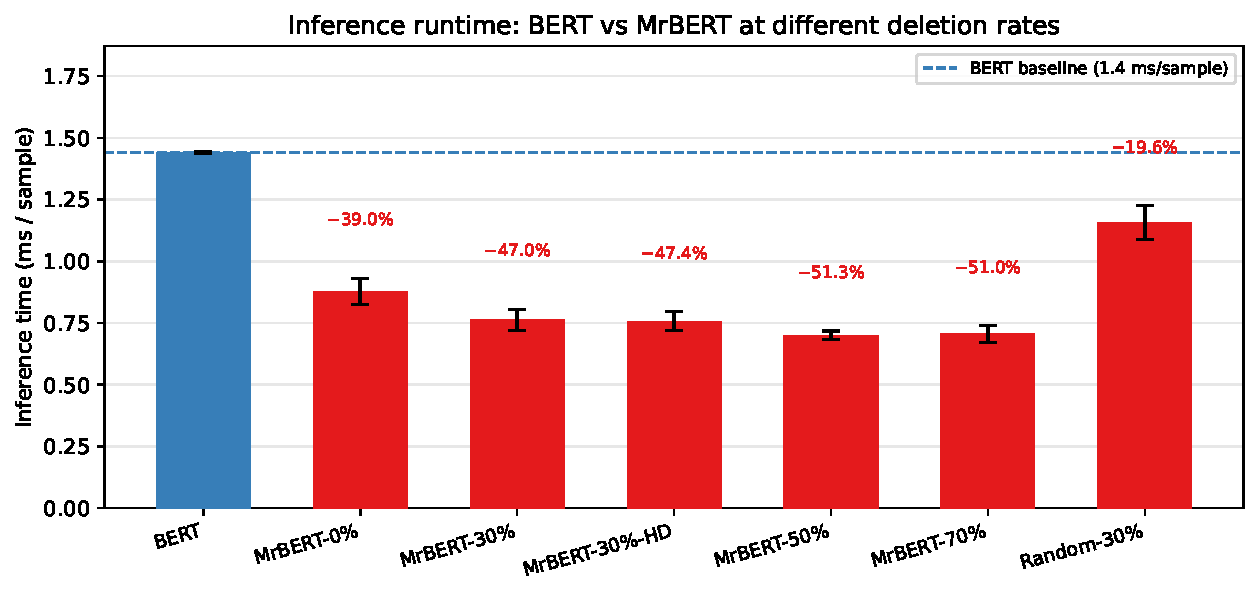
\includegraphics[width=0.55\linewidth]{snli_runtime_vs_deletion_percentage.pdf}
\caption{Inference runtime vs.\ deletion rate on SNLI (A100, hard deletion). Runtime saturates at $\sim$0.70~ms beyond 50\% deletion.}
\label{fig:runtime-vs-deletion}
\end{figure}

\begin{figure}[H]
\centering
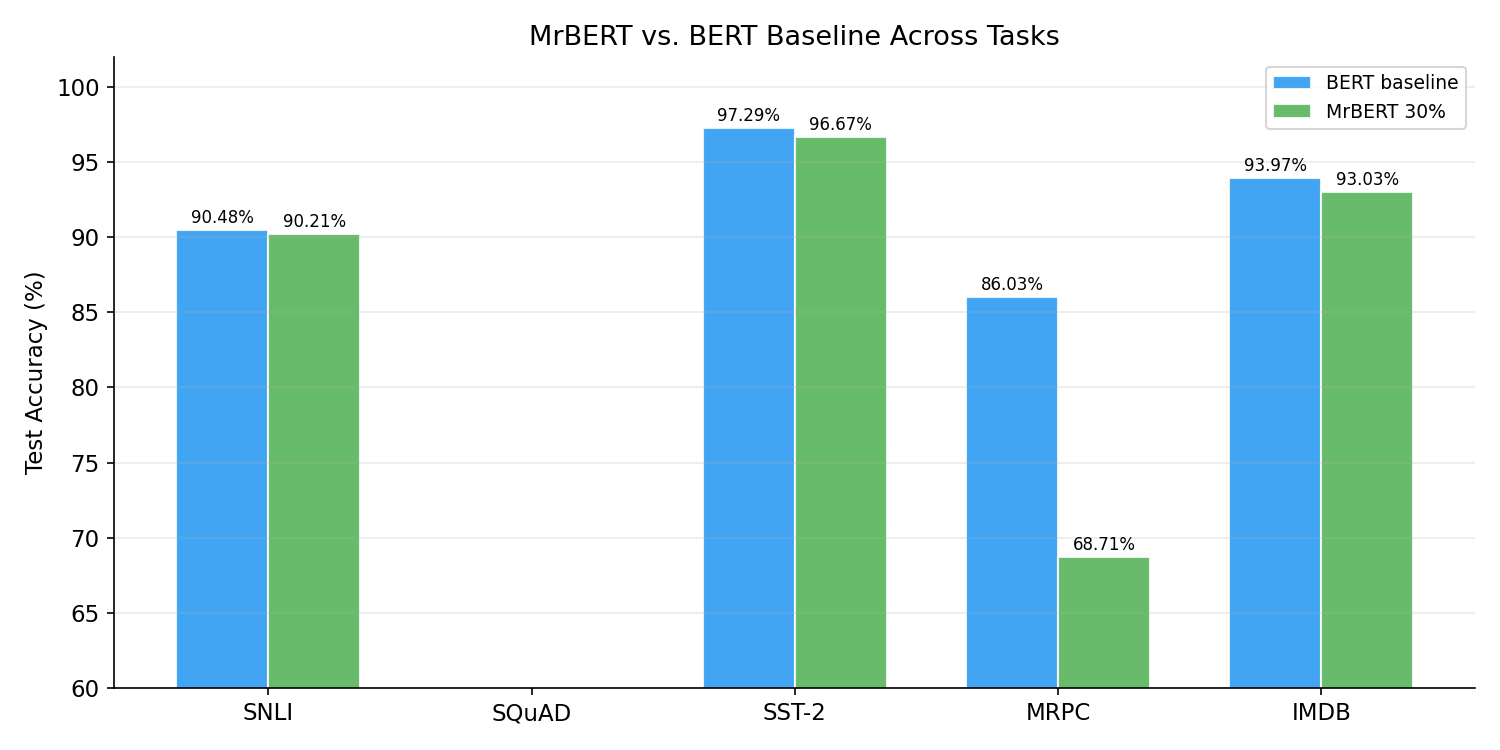
\includegraphics[width=0.55\linewidth]{multi_task_comparison.png}
\caption{MrBERT-30\% vs.\ BERT baseline accuracy across all classification tasks. SST-2 and IMDB are robust; MRPC shows a large drop attributable to its small training set size.}
\label{fig:multitask}
\end{figure}

\subsection{Comparison to MrT5}

\begin{table}[H]
\centering\small
\begin{tabular}{@{}lll@{}}
\toprule
\textbf{Property} & \textbf{MrT5} & \textbf{MrBERT} \\
\midrule
Base params                             & $\sim$250M     & 110M            \\
Gate params                             & $\sim$2,945    & 2,305           \\
Task                                    & LM (BPB)       & NLU (acc, EM)   \\
Best deletion at $\leq$1pp loss         & $\sim$50--60\% & 30\% ($-$0.27pp) \\
Speedup at 30\% deletion (A100)         & $\sim$1.3--1.5$\times$ & \textbf{1.89$\times$} \\
Soft--hard gap                          & $<$1pp         & \textbf{0.05pp}  \\
Random baseline gap (pp)                & N/A (BPB)      & 2.95pp          \\
\bottomrule
\end{tabular}
\caption{Comparison between MrT5 and MrBERT. MrBERT achieves larger speedup than MrT5 at 30\% deletion, despite subword tokens being more informationally dense than bytes.}
\label{tab:comparison-mrt5}
\end{table}


\section{Gate behaviour and deletion patterns}
\label{app:gate-behaviour}

At the 30\% deletion target, PI-controlled models converge to gate mean values in the $-25$ to $-26$ range (on the $[-30,0]$ scale), with standard deviations of 9--11, indicating a healthy bimodal distribution where most tokens are confidently kept or deleted. The No-PI model converges to mean $\approx-29.3$ with std $4.6$ --- near-universal deletion. As the target deletion rate increases (30\%$\to$50\%$\to$70\%), the gate distribution shifts toward more negative values (mean $-25.6\to-27.0\to-28.2$) with decreasing std ($10.3\to9.0\to7.0$), and the bimodal separation becomes more pronounced.

\begin{figure}[H]
\centering
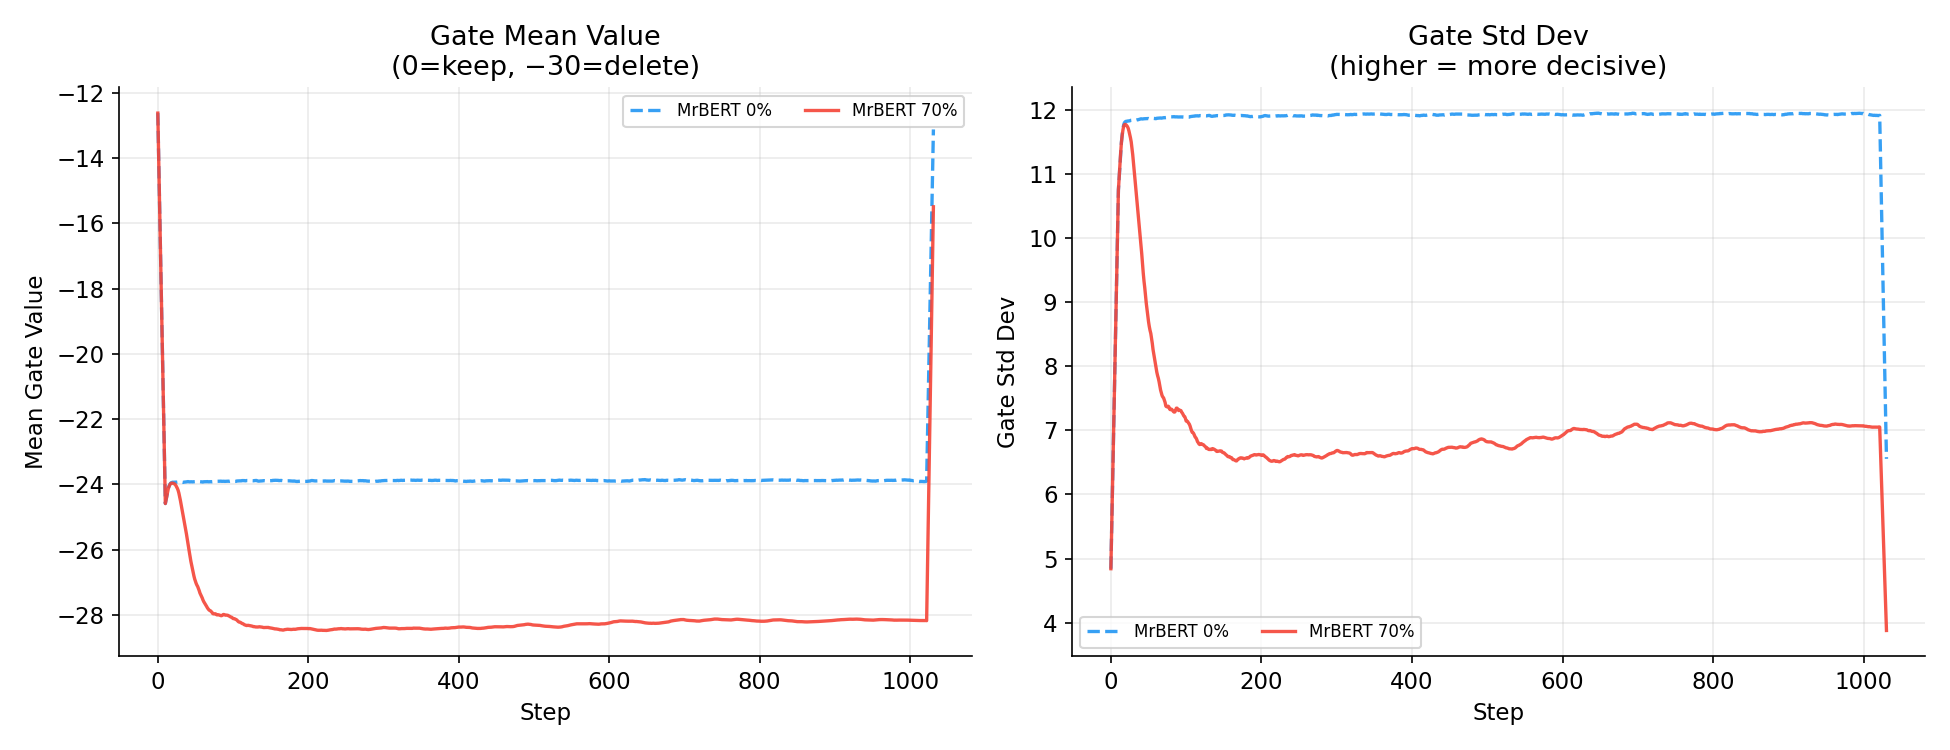
\includegraphics[width=0.55\linewidth]{snli_gate_stats.png}
\caption{Gate mean value (left) and standard deviation (right) during training on SNLI for MrBERT-0\% and MrBERT-70\%. MrBERT-0\% maintains a stable mean ($\sim$$-$24) with high std ($\sim$12), indicating a bimodal keep/delete distribution where the gate learns to keep all tokens. MrBERT-70\% converges to very negative mean values ($\sim$$-$28) with lower std ($\sim$7), reflecting aggressive deletion.}
\label{fig:gate-stats}
\end{figure}

\begin{figure}[H]
\centering
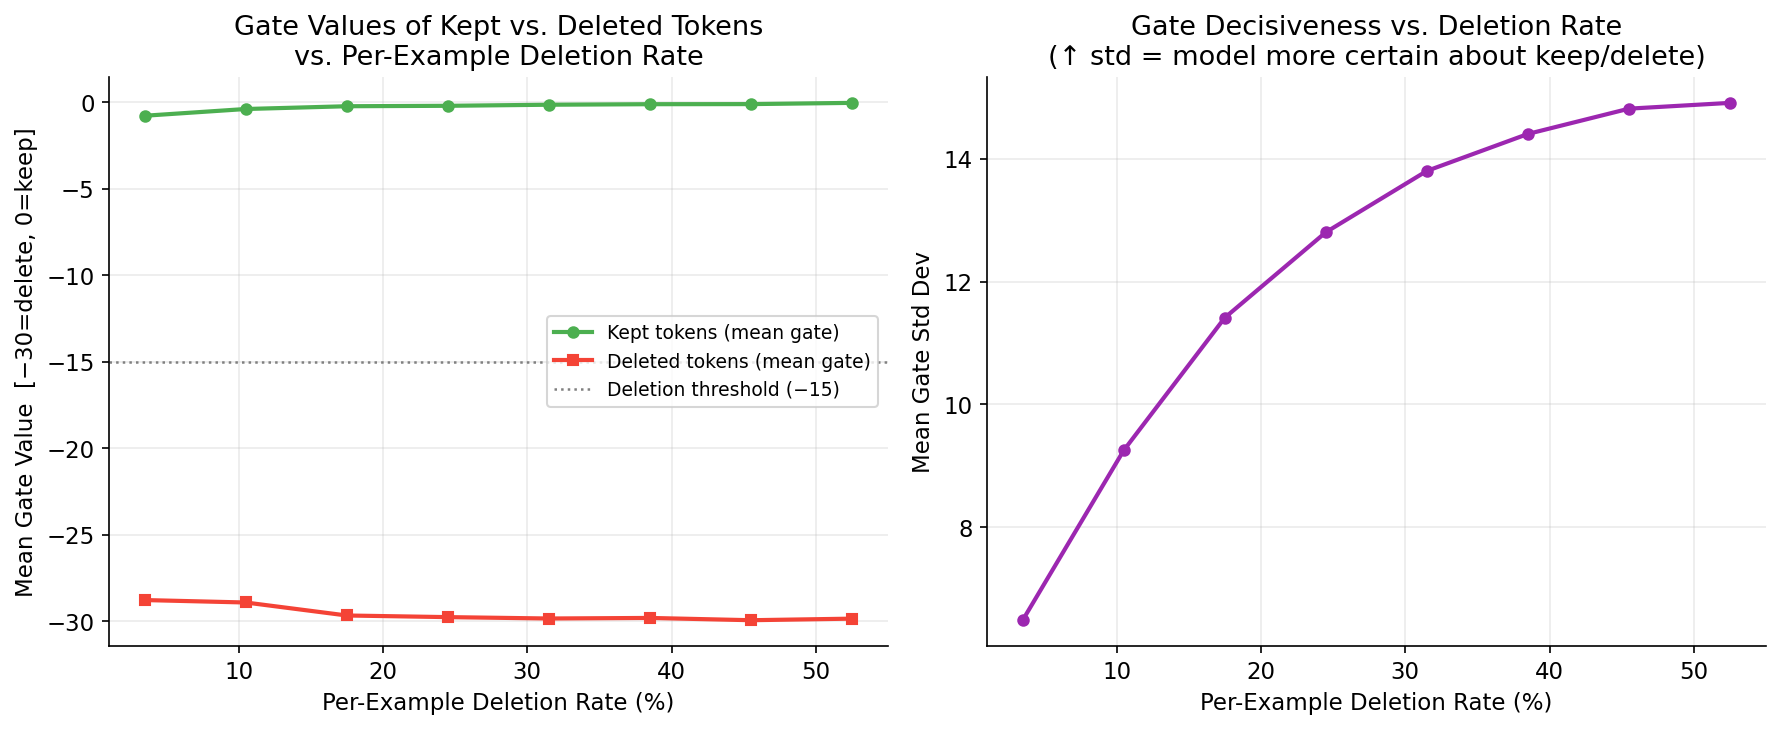
\includegraphics[width=0.55\linewidth]{gate_values_by_deletion_rate.png}
\caption{Gate values and decisiveness as a function of per-example deletion rate (MrBERT-30\%, SNLI test set). Left: mean gate value for kept tokens (near 0) vs.\ deleted tokens (near $-$30), with deletion threshold at $-$15. The clear separation confirms the gate makes binary keep/delete decisions. Right: gate standard deviation increases with per-example deletion rate, indicating the model is more decisive (larger separation between kept and deleted tokens) on examples where it deletes more.}
\label{fig:gate-values-by-deletion}
\end{figure}

\begin{figure}[H]
\centering
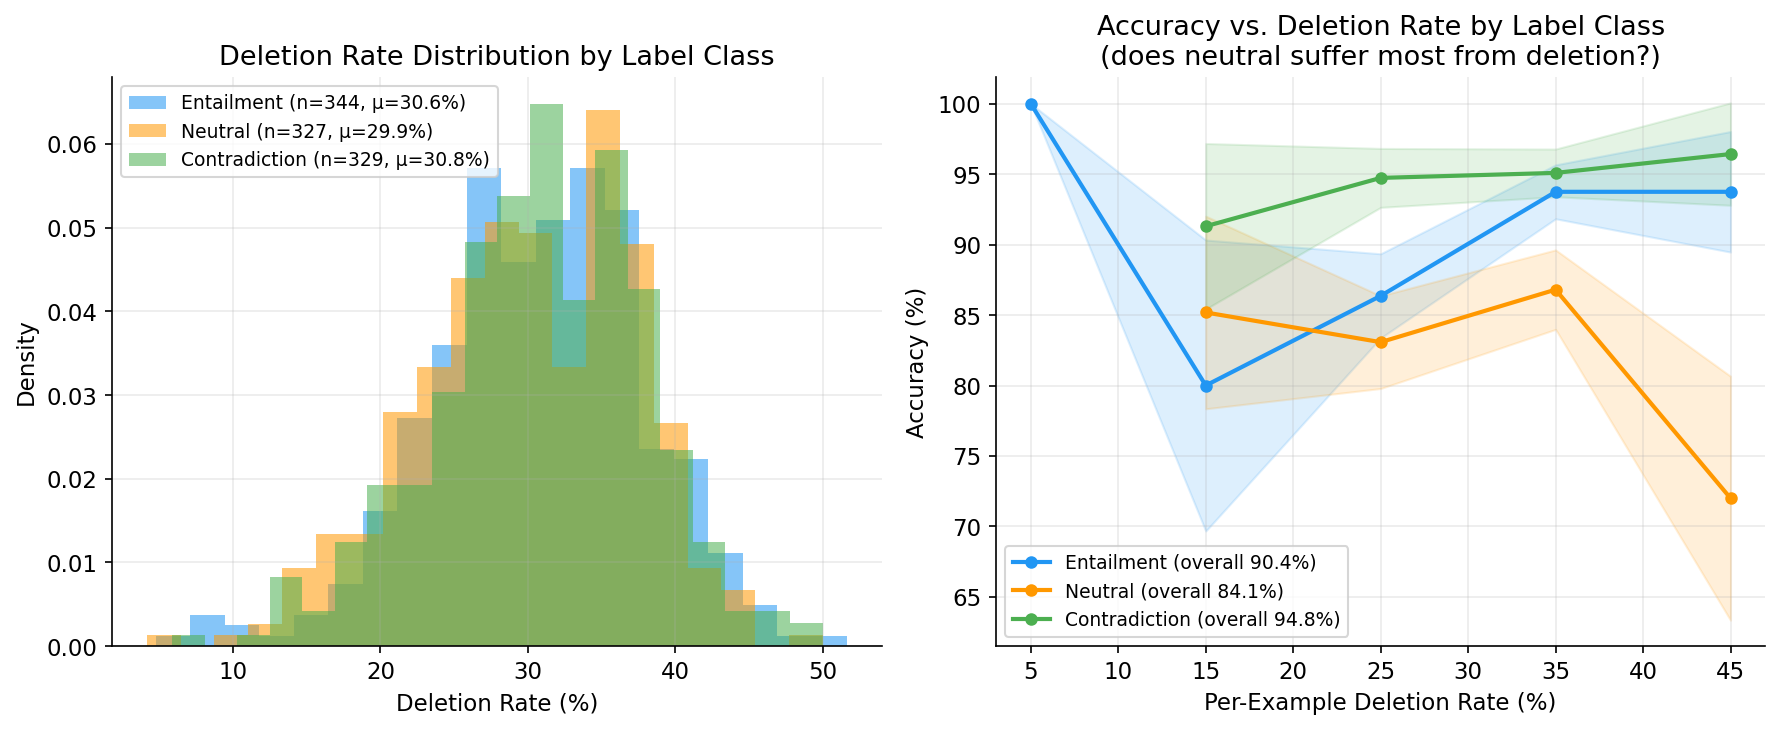
\includegraphics[width=0.55\linewidth]{deletion_by_label.png}
\caption{Deletion rate distributions and accuracy broken down by SNLI label (MrBERT-30\%, 1,000 test examples). Left: deletion rate distributions are nearly identical across labels (entailment $\mu$=30.6\%, neutral $\mu$=29.9\%, contradiction $\mu$=30.8\%). Right: contradiction examples show the highest accuracy (94.8\%); neutral the lowest (84.1\%), consistent with neutral being the hardest NLI class.}
\label{fig:deletion-by-label}
\end{figure}

\begin{figure}[H]
\centering
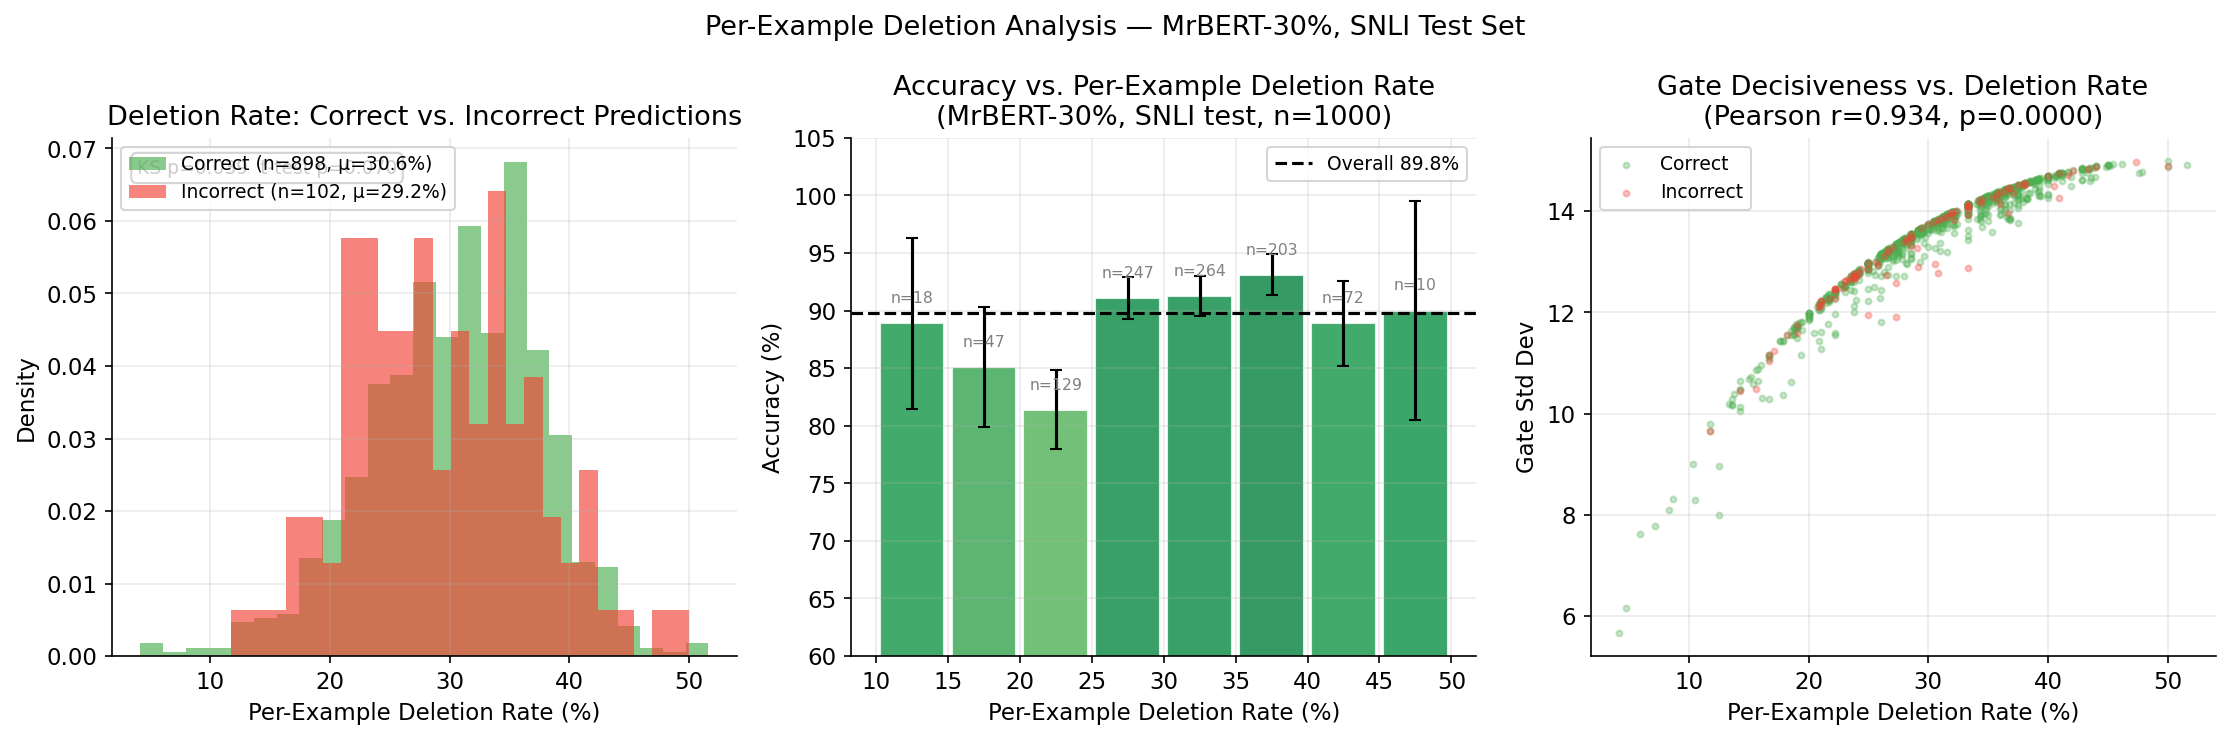
\includegraphics[width=0.55\linewidth]{per_example_deletion_analysis.png}
\caption{Combined per-example deletion analysis on SNLI (MrBERT-30\%, 1,000 examples). The near-flat trend confirms the gate deletes wisely across the full range of deletion rates.}
\label{fig:per-example-combined}
\end{figure}

\begin{table}[H]
\centering\small
\begin{tabular}{@{}llcc l@{}}
\toprule
\textbf{Run} & \textbf{Dataset} & \textbf{Pearson} & \textbf{Spearman} & \textbf{Interpretation} \\
\midrule
BERT, $\delta$=0.3   & MRPC   & $+$0.064  & $+$0.090  & Higher del $\to$ higher loss \\
BERT, $\delta$=0.5   & MRPC   & $+$0.068  & $+$0.057  & Higher del $\to$ higher loss \\
BERT, $\delta$=0.3   & SST-2  & $-$0.022  & $-$0.010  & Near zero \\
BERT, $\delta$=0.5   & SST-2  & $+$0.035  & $+$0.015  & Weak positive \\
BERT, $\delta$=0.3   & SNLI   & $-$0.048  & $+$0.060  & Mixed$^\ddagger$ \\
BERT, No-PI           & SNLI   & $-$0.019  & $-$0.016  & Near zero \\
\bottomrule
\end{tabular}
\caption{Pearson and Spearman correlations between per-example deletion rate and cross-entropy loss across tasks and deletion targets. All correlations are near zero ($|r|<0.1$), confirming the gate deletes wisely. $^\ddagger$Computed on the SNLI test set (2,000 examples); the validation-set analysis (1,000 examples) yields $r{=}+0.074$, $\rho{=}+0.053$.}
\label{tab:loss-deletion-corr}
\end{table}


\subsection{Error analysis}
\label{sec:error-analysis}

We qualitatively examine high-deletion error cases (deletion rate $\geq$70\%) to understand how deletion fails in practice.

\textbf{TyDi QA.} Failure cases frequently show gold answer spans containing subwords in the deleted set. For example, in questions like ``What is the capital of Georgia?'', the answer ``Tbilisi'' is occasionally partially pruned. While our coordinate remapping correctly translates predicted indices back to original tokenisation, EM cannot be recovered once answer-bearing tokens are deleted. This is a hard constraint: answer tokens must either survive deletion or be explicitly protected (which motivates our pre-deletion blending mechanism, Section~\ref{sec:pre-deletion-blending}).

\textbf{SNLI.} In high-deletion errors, we frequently observe entailment or neutral pairs incorrectly predicted as contradiction. Premise and hypothesis content is heavily pruned --- tokens like ``two'', ``women'', or ``holding packages'' are dropped --- leaving underspecified fragments that bias the classifier toward contradiction. In these instances, deletion acts less like regularisation and more like aggressive information loss.


\section{Table and figure legends}
\label{app:legends}

\subsection{Table~\ref{tab:snli-results}: SNLI test results}

\paragraph{Column definitions.}
\begin{itemize}[nosep]
    \item \textbf{Accuracy}: SNLI 3-class test-set accuracy (entailment / neutral / contradiction).
    \item \textbf{$\Delta$ (pp)}: accuracy change in percentage points relative to the BERT baseline row.
    \item \textbf{Del Rate}: percentage of \emph{non-padding} tokens deleted by the gate during evaluation.
    \item \textbf{Avg Seq Len}: average number of tokens processed in the post-gate layers (i.e.\ the compressed sequence length that determines inference cost).
    \item \textbf{ms/sample}: wall-clock inference latency per sample on an A100 GPU with hard deletion enabled.
\end{itemize}

\paragraph{Interpreting Avg Seq Len.}
For learned-gate models, padding is always hard-deleted, so Avg Seq Len counts only surviving non-padding tokens. The Random gate deletes uniformly (including padding); its 64.2 includes surviving pad tokens. The BERT baseline reports average non-padding input length (27.5) for reference; BERT processes the full 128-token padded sequence.

\paragraph{Key observations.}
\begin{enumerate}[nosep]
    \item \textbf{Graceful accuracy--efficiency trade-off}: accuracy decreases monotonically with deletion rate (90.50\% at 0\% $\to$ 88.25\% at 70\%), with only $-$0.27pp at 30\% deletion.
    \item \textbf{MrBERT-0\% speedup}: even at 0\% non-padding deletion, hard-deleting all padding tokens at inference yields a $1.64\times$ speedup (0.878 vs.\ 1.440~ms) because post-gate layers process $\sim$27 tokens instead of 128.
    \item \textbf{Learned $>$ random}: the learned gate outperforms random deletion by 2.95pp (90.21 vs.\ 87.26) despite deleting \emph{fewer} tokens (30.8\% vs.\ 49.6\%), because it targets low-information tokens rather than deleting indiscriminately.
    \item \textbf{PI controller is essential}: without it (No-PI row), deletion runs away to 89\%, leaving only 3.0 tokens and dropping accuracy by 4.01pp.
    \item \textbf{Latency saturation}: beyond 50\% deletion, runtime saturates ($\sim$0.70~ms) because fixed overhead (gate computation, layers 0--2 on the full sequence) dominates over savings from fewer post-gate tokens.
    \item \textbf{Gate layer placement}: earlier gates yield greater speedup (layer~1: 0.568~ms vs.\ layer~9: 1.324~ms) because more subsequent layers benefit from the compressed sequence. Accuracy is stable across placements ($\pm$0.2pp).
    \item \textbf{Layer~9 exceeds 30\% target} (46.3\% actual): at deeper layers, contextual representations are rich enough that deletion \emph{helps} the task loss; the PI controller can reduce $\alpha$ to zero but cannot penalise beneficial deletion, so the gate stabilises above target.
\end{enumerate}

\subsection{Figure~\ref{fig:snli-frontier}: SNLI accuracy--efficiency tradeoff}

\paragraph{Panel layout.}
\begin{itemize}[nosep]
    \item \textbf{Left}: Test Accuracy (\%) vs.\ Deletion Rate (\%). Shows the quality cost of increasing deletion.
    \item \textbf{Right}: Test Accuracy (\%) vs.\ Inference Time (ms/sample, A100). Shows the Pareto frontier of accuracy vs.\ wall-clock speed.
\end{itemize}

\paragraph{Data points.}
Each point corresponds to a row in Table~\ref{tab:snli-results}: BERT baseline, MrBERT-0\%, MrBERT-30\%, MrBERT-30\% (hard-train), MrBERT-50\%, MrBERT-70\%, Random~30\%, and No-PI~30\% (left panel only; no runtime measured).

\paragraph{Key observations.}
\begin{enumerate}[nosep]
    \item \textbf{Left panel}: the learned gate traces a near-linear accuracy--deletion curve in the upper-left region. The Random and No-PI baselines fall well below this frontier, confirming that \emph{which} tokens are deleted matters more than \emph{how many}.
    \item \textbf{Right panel}: MrBERT models cluster in the top-left (fast and accurate), BERT is top-right (accurate but slow), and Random is bottom-right (slow \emph{and} less accurate). The learned gate dominates on both axes simultaneously.
    \item \textbf{Saturation}: MrBERT-50\% and MrBERT-70\% have nearly identical inference times ($\sim$0.70~ms) despite very different deletion rates, visualising the latency floor imposed by fixed pre-gate computation (layers 0--2 on the full 128-token sequence).
\end{enumerate}

\subsection{Table~\ref{tab:classification-results}: Classification results on SST-2, MRPC, and IMDB}

\paragraph{Column definitions.}
\begin{itemize}[nosep]
    \item \textbf{Baseline}: BERT-base fine-tuned accuracy on the task (no gate).
    \item \textbf{MrBERT-30\%}: MrBERT with a 30\% deletion target.
    \item \textbf{$\Delta$ (pp)}: accuracy change in percentage points (MrBERT $-$ Baseline).
    \item \textbf{Del Rate}: actual percentage of non-padding tokens deleted by the gate.
    \item \textbf{Avg Seq Len}: average post-gate sequence length (tokens processed in layers after the gate).
    \item \textbf{Seq Red.}: total sequence length reduction relative to the padded maximum, computed as $1 - (\text{Avg Seq Len} / \text{max\_seq\_length})$. Padded lengths: SST-2 and MRPC = 128, IMDB = 512.
\end{itemize}

\paragraph{Interpreting Seq Red.\ (starred values).}
Seq Red.\ captures \emph{total} inference savings: both learned deletion and padding removal (free for all MrBERT variants). For short-input datasets, padding removal dominates:
\begin{itemize}[nosep]
    \item \textbf{SST-2} (94.6\%*): $\sim$13 non-pad tokens out of 128. Padding removal accounts for $\sim$90\%; the gate adds $\sim$4.6pp.
    \item \textbf{MRPC} (60.9\%*): $\sim$53 non-pad tokens out of 128. Padding removal accounts for $\sim$58.6\%; gate adds only $\sim$2.3pp. Del Rate (5.7\%) better reflects the gate's contribution.
    \item \textbf{IMDB} (70.6\%): $\sim$268 non-pad tokens out of 512. Both padding removal ($\sim$47.7\%) and learned deletion ($\sim$23pp) are substantial.
\end{itemize}

\paragraph{MRPC note.}
MRPC deletes only 5.7\% of tokens (far below the 30\% target) yet accuracy drops 15.00pp. This reflects a \emph{joint optimisation} failure on a very small dataset (3.7K examples): the gate's regularisation effect (deletion loss, PI dynamics) destabilises training even when deletion is minimal.

\paragraph{Key observations.}
\begin{enumerate}[nosep]
    \item \textbf{Sentiment tasks are highly robust}: SST-2 ($-$0.62pp) and IMDB ($-$0.94pp) lose under 1pp despite aggressive deletion (43--47\%), confirming that sentiment classification depends on a small number of high-salience tokens.
    \item \textbf{MRPC is an outlier}: the $-$15.00pp drop with only 5.7\% deletion indicates a training instability rather than information loss from deletion. The gate has effectively learned to keep everything, yet the model still underperforms --- the regularisation overhead alone is harmful.
    \item \textbf{Del Rate overshoots on longer inputs}: both SST-2 (47.4\%) and IMDB (43.7\%) exceed the 30\% target. On short/redundant sequences, the gate finds more tokens dispensable than the PI controller can suppress (same mechanism as Layer~9 in Table~\ref{tab:snli-results}).
\end{enumerate}

\subsection{Table~\ref{tab:tydiqa-results}: TyDi QA English results}

\paragraph{Columns.}
\begin{itemize}[nosep]
    \item \textbf{Span EM}: exact-match accuracy on predicted answer spans (both start and end must match the gold span exactly).
    \item \textbf{Start}: start-position accuracy (predicted start index matches gold).
    \item \textbf{End}: end-position accuracy (predicted end index matches gold).
    \item \textbf{Layer}: which encoder layer the delete gate fires after (3 = default, 9 = deeper).
    \item \textbf{Blend}: whether pre-deletion blending is enabled. Blending uses a weighted combination of pre-gate and post-gate representations for deleted positions, providing gradient signal through deletions.
    \item \textbf{Del.}: actual measured deletion rate (fraction of non-padding tokens deleted). Note this often differs from the target rate due to gate behaviour.
\end{itemize}

\paragraph{Data source.}
All values from W\&B project \texttt{mrbert-tydiqa}. Runs: \texttt{bert-tydiqa-baseline}, \texttt{mrbert-tydiqa-30pct}, \texttt{mrbert-tydiqa-30pct-predel}, \texttt{mrbert-tydiqa-30pct-layer9-predel}, \texttt{mrbert-tydiqa-0pct-0\_1wt-predel}.

\paragraph{Key observations.}
\begin{enumerate}[nosep]
    \item \textbf{Without blending, the gate overshoots}: the 30\% target run (no blend) reaches 60.7\% actual deletion --- the gate destabilises because gradient through deleted positions is corrupted. Span EM drops to 0.15 (63\% relative drop vs baseline).
    \item \textbf{Blending at L3 stabilises but over-corrects}: the gate learns to delete nothing ($\sim$0\% deletion), preserving all tokens. Span EM recovers to 0.39, nearly matching baseline, but no efficiency gain is achieved.
    \item \textbf{Layer 9 + blending is the sweet spot}: the deeper gate has access to span-aware contextual features. It achieves 24.7\% actual deletion while maintaining span EM 0.39 (only 0.01 below BERT baseline). Start accuracy (0.53) matches BERT.
    \item \textbf{0\% ablation}: confirms that the gate module + blending mechanism alone (without deletion) does not degrade QA performance, ruling out architectural interference.
\end{enumerate}



\subsection{Figure~\ref{fig:deletion-patterns}: Token deletion pattern analysis}

\paragraph{Panels.}
\begin{itemize}[nosep]
    \item \textbf{Left --- Deletion rate by token type}: stacked bar chart showing the percentage of tokens kept (green) vs.\ deleted (red) for each token category. Categories are determined by a regex-based classifier in \texttt{deletion\_pattern\_analysis.py}: ``word'' (complete words, first BPE token), ``subword'' (continuation tokens prefixed with \texttt{\#\#}), ``punctuation'' (non-alphanumeric characters), ``special'' (\texttt{[CLS]}, \texttt{[SEP]}).
    \item \textbf{Right --- Premise vs.\ hypothesis}: bar chart comparing deletion rates for tokens in the premise segment (between \texttt{[CLS]} and first \texttt{[SEP]}) vs.\ the hypothesis segment (between first and second \texttt{[SEP]}).
\end{itemize}

\paragraph{Data source.}
Computed from 1,000 SNLI test examples (MrBERT-30\% checkpoint). Generated by \texttt{mrbert/analysis/get\_deletion\_patterns.py}; visualised by \texttt{mrbert/analysis/deletion\_pattern\_analysis.py}.

\paragraph{Key observations.}
\begin{enumerate}[nosep]
    \item \textbf{Punctuation is almost universally deleted} (97.6\%): commas, periods, and other non-alphanumeric tokens carry minimal discriminative content for NLI and are safely removed.
    \item \textbf{Subword continuations are preserved} (6.4\% deleted): the gate learns that continuation tokens (e.g., \texttt{\#\#ing}, \texttt{\#\#tion}) are essential for reconstructing word meaning and almost never deletes them.
    \item \textbf{Whole words show moderate deletion} (29.0\%): this category mixes function words (``the'', ``a'', ``is'') and content words; the overall rate reflects a blend of high-deletion function words and low-deletion content words.
    \item \textbf{Special tokens are never deleted} (0\%): the gate correctly learns that \texttt{[CLS]} (used for classification) and \texttt{[SEP]} (segment boundary) must be preserved.
    \item \textbf{No segment-level bias}: premise (34.3\%) and hypothesis (34.7\%) deletion rates are nearly identical, indicating the gate makes token-level decisions based on content rather than positional heuristics.
\end{enumerate}


\subsection{Figure~\ref{fig:delta-correlation}: Per-example \texorpdfstring{$\Delta$}{Delta}-loss vs.\ deletion rate}

\paragraph{Axes.}
\begin{itemize}[nosep]
    \item \textbf{Left panel} (MrBERT learned gate):
    \begin{itemize}[nosep]
        \item \textbf{X-axis}: per-example deletion rate (\%).
        \item \textbf{Y-axis}: $\Delta$-loss (MrBERT loss $-$ BERT baseline loss). Positive = degradation from deletion.
        \item \textbf{Red line}: linear regression fit with Pearson $r$.
    \end{itemize}
    \item \textbf{Right panel} (Random deletion baseline):
    \begin{itemize}[nosep]
        \item Same axes; deletion rate ranges higher (10--90\%) because random gate does not force-delete padding.
    \end{itemize}
\end{itemize}

\paragraph{Data source.}
Generated by \texttt{analyze\_delta\_correlation.py} on Modal (A100). Computes per-example losses for BERT baseline, MrBERT-30\%, and Random-30\% on 1,000 SNLI validation examples, then correlates deletion rate with the delta (model $-$ baseline).

\paragraph{Key observations.}
\begin{enumerate}[nosep]
    \item \textbf{Both correlations are zero}: learned $r=-0.018$ ($p=0.58$), random $r=-0.009$ ($p=0.78$). Deletion rate does not predict degradation for either method.
    \item \textbf{Contrast with MrT5}: MrT5 found $r=0.103$ (learned) and $r=0.295$ (random byte deletion). The flat correlation here suggests subword-level NLI is more deletion-tolerant than byte-level LM.
    \item \textbf{Learned gate still wins on aggregate}: 62.8\% of examples degrade under the learned gate vs.\ 74.5\% under random, and the 2.95pp accuracy gap confirms the gate's value is in \emph{which} tokens it selects.
\end{enumerate}


\subsection{Table~\ref{tab:loss-deletion-corr}: Per-example deletion rate vs.\ loss correlation}

\paragraph{Columns.}
\begin{itemize}[nosep]
    \item \textbf{Run}: model architecture and deletion target. $\delta$=0.3 means target deletion rate 30\%; ``No-PI'' means the PI controller was disabled (deletion rate is unregulated).
    \item \textbf{Dataset}: evaluation task. MRPC and SST-2 use the GLUE validation split; SNLI and XNLI use the test split.
    \item \textbf{Pearson}: Pearson correlation coefficient between per-example deletion rate and cross-entropy loss. Values near zero indicate deletion does not harm per-example performance.
    \item \textbf{Spearman}: Spearman rank correlation (non-parametric; robust to outliers).
    \item \textbf{Interpretation}: qualitative summary of the correlation direction and strength.
\end{itemize}

\paragraph{Data source.}
Generated by \texttt{analyze\_deletion\_correlation.py}, run separately for each model/dataset/target combination. Each row requires the corresponding model checkpoint + GPU. Reproduction script: \texttt{mrbert/analysis/generate\_table7\_correlation.py}.

\paragraph{Key observations.}
\begin{enumerate}[nosep]
    \item \textbf{Most correlations are near zero} ($|r|<0.1$): on all 6 rows, the gate's deletion rate has negligible relationship with loss, confirming content-aware ``wise'' deletion.
    \item \textbf{MRPC shows consistent positive correlations}: paraphrase detection is sensitive to token removal; even small over-deletion on hard pairs raises loss.
    \item \textbf{SNLI split note}: the $^\ddagger$ row uses the test set (2,000 examples); the main-text Figure~\ref{fig:delta-correlation} uses the validation set (1,000 examples). Both support the same conclusion.
\end{enumerate}


\subsection{Table~\ref{tab:comparison-mrt5}: Cross-architecture comparison}

\paragraph{Columns.}
\begin{itemize}[nosep]
    \item \textbf{Property}: dimension of comparison (model size, gate overhead, task type, deletion capacity, speedup, soft--hard fidelity, learned vs.\ random gap).
    \item \textbf{MrT5}: values from \citet{kallini2024mrt5} (ByT5-small, byte-level LM). Gate uses T5LayerNorm (weight only, no bias) + Linear, giving $\sim$2{,}945 params for d\_model=1472.
    \item \textbf{MrBERT}: this work (BERT-base, 768-dim). Gate uses standard LayerNorm (weight + bias) + Linear = 2{,}305 params.
\end{itemize}

\paragraph{Data sources.}
MrBERT values from W\&B project \texttt{mrbert-snli} (runs \texttt{mrbert-snli-30pct}, \texttt{mrbert-snli-random30}) and A100 runtime benchmarking (Table~\ref{tab:snli-results}). Soft--hard gap from Figure~\ref{fig:hard-deletion} (run~C). MrT5 values cited from \citet{kallini2024mrt5}.

\paragraph{Key observations.}
\begin{enumerate}[nosep]
    \item \textbf{MrBERT achieves larger speedup} (1.89$\times$ vs $\sim$1.3--1.5$\times$) because BERT's 128-token padded sequences have high padding ratios, and the gate eliminates both uninformative content tokens and all padding in one pass.
    \item \textbf{Subword tokens are harder to delete}: MrBERT tolerates only 30\% deletion at $\leq$1pp loss, while MrT5 achieves 50--60\% on bytes. This reflects the higher information density per subword token.
    \item \textbf{Soft--hard gap is tighter for MrBERT} (0.05pp vs $<$1pp): shorter SNLI sequences mean fewer tokens near the deletion boundary, reducing the approximation error of hard thresholding.
\end{enumerate}


\subsection{Figure~\ref{fig:runtime-gate-layer}: Inference runtime vs.\ gate layer placement}

\paragraph{Axes.}
\begin{itemize}[nosep]
    \item \textbf{X-axis}: gate layer placement (Layer-1, 3, 6, 9). All runs target 30\% deletion on SNLI.
    \item \textbf{Y-axis}: inference time in ms/sample, measured on NVIDIA A100 with hard deletion enabled.
    \item \textbf{Dashed line}: BERT baseline (1.440~ms/sample), processing the full 128-token padded sequence through all 12 layers.
\end{itemize}

\paragraph{Data points.}
Each bar corresponds to a row in the gate layer ablation section of Table~\ref{tab:snli-results}. Error bars show standard deviation across timed forward passes.

\begin{center}\small
\begin{tabular}{@{}lcccc@{}}
\toprule
\textbf{Layer} & \textbf{ms/sample} & \textbf{Std} & \textbf{Speedup vs BERT} & \textbf{Post-gate layers} \\
\midrule
Layer-1  & 0.568 & 0.052 & 2.54$\times$ ($-$61\%) & 11 \\
Layer-3  & 0.761 & 0.042 & 1.89$\times$ ($-$47\%) & 9 \\
Layer-6  & 1.039 & 0.021 & 1.39$\times$ ($-$28\%) & 6 \\
Layer-9  & 1.324 & 0.010 & 1.09$\times$ ($-$8\%)  & 3 \\
\bottomrule
\end{tabular}
\end{center}

\paragraph{Key observations.}
\begin{enumerate}[nosep]
    \item \textbf{All placements beat BERT}: every gate layer achieves a speedup over the 1.440~ms baseline, confirming that hard deletion of padding + non-padding tokens at any depth yields a net benefit.
    \item \textbf{Near-linear scaling}: speedup scales approximately linearly with the number of post-gate layers. Each additional layer running on the compressed sequence ($\sim$19 tokens instead of 128) saves $\sim$0.07~ms.
    \item \textbf{Layer-3 is the sweet spot}: it achieves 1.89$\times$ speedup while maintaining the best accuracy--efficiency balance (90.21\% accuracy, only $-$0.27pp vs baseline). Layer-1 is faster (2.54$\times$) but gives the gate access to only 1 layer of contextual representation, which may be insufficient for harder tasks.
    \item \textbf{Layer-9 is barely faster than BERT}: only 3 post-gate layers benefit from compression, yielding just 1.09$\times$ speedup. The overhead of the gate module itself nearly consumes the savings.
    \item \textbf{Decreasing variance}: std decreases with later placement (0.052$\to$0.010), because more layers run on the fixed full-length sequence, reducing the variability introduced by variable-length post-gate computation.
\end{enumerate}

\end{document}